\documentclass[12pt,a4paper]{article}
\usepackage[a4paper, margin=0.8in, headheight=14pt]{geometry}
\usepackage{fontspec}
\usepackage{unicode-math}
\setmainfont{TeX Gyre Pagella}
\setmonofont[Scale=0.88]{TeX Gyre Cursor}
\setmathfont{Latin Modern Math}
\usepackage{xcolor}
\usepackage{colortbl}
\usepackage{titlesec}
\usepackage{enumitem}
\usepackage{tabularx}
\usepackage{booktabs}
\usepackage{array}
\usepackage{amsmath}
\allowdisplaybreaks
\usepackage{tikz}
\usetikzlibrary{shapes.geometric, arrows.meta, positioning, calc, fit, decorations.pathreplacing, decorations.pathmorphing, patterns, backgrounds}
% circuitikz not required for this subject
\usepackage{tcolorbox}
\tcbuselibrary{skins, breakable}
\usepackage{etoolbox}
\usepackage{hyperref}
\usepackage{fancyhdr}
\usepackage{graphicx}
\usepackage{microtype}
\hyphenpenalty=10000
\exhyphenpenalty=10000
\sloppy
\usepackage{caption}
\usepackage{setspace}
\usepackage{multirow}
\usepackage{tocloft}
\newcommand{\Q}[1]{\textbf{#1}\par\noindent\ignorespaces}
\definecolor{myred}{RGB}{196,30,58}
\definecolor{mydark}{RGB}{30,30,50}
\definecolor{mygreen}{RGB}{14,120,80}
\definecolor{myteal}{RGB}{0,130,140}
\definecolor{myamber}{RGB}{180,100,0}
\definecolor{mypurple}{RGB}{100,30,160}
\definecolor{mygray}{RGB}{246,247,249}
\definecolor{mgframe}{RGB}{180,185,200}
\definecolor{watermark}{RGB}{145,150,170}
\definecolor{hdrred}{RGB}{250,232,235}
\definecolor{hdrgreen}{RGB}{220,244,233}
\definecolor{hdrteal}{RGB}{220,242,244}
\definecolor{hdramber}{RGB}{253,242,215}
\definecolor{hdrpurple}{RGB}{238,228,255}
\definecolor{hdrgray}{RGB}{238,240,245}
\AfterEndEnvironment{tcolorbox}{\color{mydark}}

\titleformat{\section}{\large\bfseries\color{myred}}{\thesection.}{0.5em}{}[\vspace{1pt}{\color{myred}\rule{\linewidth}{0.8pt}}]
\titleformat{\subsection}{\normalsize\bfseries\color{myteal}}{\thesubsection}{0.5em}{}
\titlespacing*{\section}{0pt}{18pt}{7pt}
\titlespacing*{\subsection}{0pt}{11pt}{4pt}
\setlength{\parindent}{0pt}
\setlength{\parskip}{4pt}
\renewcommand{\cfttoctitlefont}{\large\bfseries\color{myred}}
\renewcommand{\cftaftertoctitle}{\par\noindent{\color{myred}\rule{\linewidth}{0.8pt}}}
\setlength{\cftbeforetoctitleskip}{0pt}
\setlength{\cftaftertoctitleskip}{6pt}
\renewcommand{\cftsecfont}{\normalsize\bfseries\color{mydark}}
\renewcommand{\cftsecpagefont}{\normalsize\bfseries\color{mydark}}
\renewcommand{\cftsecleader}{\cftdotfill{\cftdotsep}}
\setlength{\cftbeforesecskip}{5pt}
\renewcommand{\cftsubsecfont}{\small\color{mydark}}
\renewcommand{\cftsubsecpagefont}{\small\color{mydark}}
\setlength{\cftbeforesubsecskip}{2pt}
\setlength{\cftsubsecindent}{1.4em}
\renewcommand{\cftpartfont}{\normalsize\bfseries\color{myteal}}
\renewcommand{\cftpartpagefont}{\normalsize\bfseries\color{myteal}}
\setlength{\cftbeforepartskip}{10pt}
\renewcommand{\arraystretch}{1.45}
\setlength{\tabcolsep}{6pt}
\arrayrulecolor{mydark}
\newcolumntype{B}[1]{>{\small\bfseries\raggedright\arraybackslash}m{#1}}
\newcolumntype{C}[1]{>{\centering\arraybackslash}m{#1}}
\newcolumntype{Y}{>{\small\raggedright\arraybackslash}X}
\renewcommand{\tabularxcolumn}[1]{m{#1}}
\newcommand{\currmodule}{Module 1}
\pagestyle{fancy}
\fancyhf{}
\fancyhead[L]{\small\color{myred}\textbf{BS-B401}\;\color{mydark}--- Biology for Engineers}
\fancyhead[R]{\small\color{myteal}\textbf{\currmodule\ Notes}}
\fancyfoot[C]{\small\color{mydark}\thepage}
\fancyfoot[R]{\small\color{watermark}\textit{\copyright\ Biraj}}
\renewcommand{\headrulewidth}{0.5pt}
\renewcommand{\footrulewidth}{0.3pt}

\hypersetup{colorlinks=true, linkcolor=myteal, urlcolor=myteal,
  pdfauthor={Biraj Sarkar},
  pdftitle={BS-B401 --- Combined Notes}}

\tcbset{
  tikzbox/.style={
    colback=mygray, colframe=mgframe, boxrule=0.6pt, arc=4pt,
    left=8pt, right=8pt, top=6pt, bottom=6pt,
    colbacktitle=mgframe, coltitle=mydark, fonttitle=\small\bfseries
  },
  defbox/.style={
    colback=hdrgreen, colframe=mygreen, boxrule=0.8pt, arc=4pt,
    left=9pt, right=9pt, top=6pt, bottom=6pt,
    colbacktitle=mygreen, coltitle=white, fonttitle=\small\bfseries
  },
  formulabox/.style={
    colback=hdrteal, colframe=myteal, boxrule=0.8pt, arc=4pt,
    left=9pt, right=9pt, top=7pt, bottom=7pt,
    colbacktitle=myteal, coltitle=white, fonttitle=\small\bfseries
  },
  examplebox/.style={
    colback=hdramber, colframe=myamber, boxrule=0.8pt, arc=4pt,
    left=9pt, right=9pt, top=6pt, bottom=6pt,
    colbacktitle=myamber, coltitle=white, fonttitle=\small\bfseries
  },
  masonbox/.style={
    colback=hdrpurple, colframe=mypurple, boxrule=0.8pt, arc=4pt,
    left=9pt, right=9pt, top=6pt, bottom=6pt,
    colbacktitle=mypurple, coltitle=white, fonttitle=\small\bfseries
  },
  exambox/.style={
    colback=hdrpurple, colframe=mypurple, boxrule=1pt, arc=5pt,
    left=10pt, right=10pt, top=8pt, bottom=8pt,
    colbacktitle=mypurple, coltitle=white, fonttitle=\bfseries,
    breakable, title after break={\textbf{Frequently Asked / Viva Questions (contd.)}}
  }
}
\tcbset{breakable}
\tcbset{coltext=mydark}
\tcbset{after={\color{mydark}}}

\tikzset{
  block/.style={rectangle, draw=myteal, fill=hdrteal,
    text width=2.4cm, align=center, minimum height=0.95cm,
    font=\small, rounded corners=3pt, line width=0.7pt},
  redblock/.style={rectangle, draw=myred, fill=hdrred,
    text width=2.4cm, align=center, minimum height=0.95cm,
    font=\small, rounded corners=3pt, line width=0.7pt},
  amberblock/.style={rectangle, draw=myamber, fill=hdramber,
    text width=2.4cm, align=center, minimum height=0.95cm,
    font=\small, rounded corners=3pt, line width=0.7pt},
  sumjunc/.style={circle, draw=myamber, fill=hdramber,
    minimum size=0.62cm, font=\small, line width=0.8pt},
  arrow/.style={-Stealth, thick, color=mydark},
  redarrow/.style={-Stealth, thick, color=myred},
  line/.style={thick, color=mydark}
}

\newcommand{\modulestart}[2]{%
  \clearpage
  \renewcommand{\currmodule}{Module #1}%
  \renewcommand{\theHsection}{mod#1.\arabic{section}}%
  \renewcommand{\theHsubsection}{\theHsection.\arabic{subsection}}%
  \renewcommand{\theHsubsubsection}{\theHsubsection.\arabic{subsubsection}}%
  \phantomsection
  \addcontentsline{toc}{part}{Module #1: #2}%
  \setcounter{section}{0}%
  \begin{center}
    \vspace*{1.0cm}
    {\Huge\bfseries\color{myred} Module #1}\\[10pt]
    {\Large\bfseries\color{mydark} #2}\\[10pt]
    {\color{myred}\rule{0.55\linewidth}{1.2pt}}
  \end{center}
  \vspace{14pt}
}
\begin{document}

\thispagestyle{empty}

% ─── Page Border (TikZ Overlay) ────────────────────────────────────────────────
\begin{tikzpicture}[remember picture, overlay]
  % Outer border (fine line in mgframe)
  \draw[color=mgframe, line width=1.5pt] 
    ($(current page.north west) + (0.6in, -0.6in)$) rectangle 
    ($(current page.south east) + (-0.6in, 0.6in)$);
  % Inner border (finer accent line in myred)
  \draw[color=myred, line width=0.8pt] 
    ($(current page.north west) + (0.65in, -0.65in)$) rectangle 
    ($(current page.south east) + (-0.65in, 0.65in)$);
\end{tikzpicture}

\vspace*{1.0cm}
\begin{center}
  {\Huge\bfseries\color{myred} BS-B401}\\[10pt]
  {\LARGE\bfseries\color{mydark} Biology for Engineers}\\[20pt]
  {\color{myred}\rule{0.7\linewidth}{1.5pt}}\\[18pt]
  {\Large\color{myteal}\textbf{Combined Module Notes}}\\[8pt]
  {\large\color{mydark} Modules 1 -- 9}\\[40pt]
  {\normalsize\color{mydark} Semester IV \quad$\bullet$\quad ECE \quad$\bullet$\quad 3 Credits}\\[12pt]
  {\normalsize\color{mydark} CGEC \;$|$\; B.Tech ECE (2023--27)}
\end{center}
\vspace{1.0cm}
\begin{center}
  \begin{tcolorbox}[colback=mygray, colframe=mgframe, boxrule=0.5pt, arc=3pt, width=0.85\linewidth]
    \centering\small\color{mydark}
    \textbf{Disclaimer / Study Guide Notice:}\\
    These are condensed \textbf{Short Notes} focusing on core theory, key formulas, block/circuit diagrams, and standard viva Q\&As for university exam revision. Exhaustive numerical practice problems and derivation edge cases are not covered. This serves as a quick-revision reference guide for students.
  \end{tcolorbox}
\end{center}
\vfill
\vspace{0.6cm}
\begin{center}
  {\large\bfseries\color{mypurple} Biraj Sarkar}\\[16pt]
  {\footnotesize\color{watermark}\textbf{IN ASSOCIATION WITH}}\\[8pt]
  {\small\bfseries\color{mydark} MAKAUT Wingman \quad$\bullet$\quad MAKAUT Future Minds}\\[12pt]
  {\large\bfseries\color{myteal} Cooch Behar Government Engineering College}
\end{center}
\vfill
\begin{center}{\small\color{watermark}\textit{Exam-Ready Notes}}\end{center}
\clearpage

\hypersetup{linkcolor=mydark}
\tableofcontents
\hypersetup{linkcolor=myteal}
\clearpage

% -- Module 1 -----------------------------------------------------------------
\modulestart{1}{Biology and Engineering}

\section{Biology and Engineering}
\subsection{How science and engineering ask different questions}
\begin{tcolorbox}[defbox, title={Biology}]
Biology is the scientific study of living systems. It asks how organisms are built, how they work, how they inherit characteristics, and how they interact and evolve. It uses evidence and quantitative reasoning alongside physics, chemistry and mathematics.
\end{tcolorbox}

\par\vspace{5pt}
\begingroup
\setlength{\extrarowheight}{1pt}
\noindent\begin{tabularx}{\linewidth}{|B{3cm}|Y|Y|}
\hline
\textbf{Question} & \textbf{Scientific approach} & \textbf{Engineering approach} \\ \hline
Purpose & Explain and predict a natural phenomenon. & Design a solution that meets a specified need. \\ \hline
Starting point & Observe a pattern and form a testable hypothesis. & Set a goal, performance criteria and constraints. \\ \hline
Evidence & Compare predictions with measurements, controls and repeated observations. & Test a prototype against requirements for performance, cost, reliability or safety. \\ \hline
Outcome & A model that may be revised when new evidence arrives. & A design that may be revised when tests reveal a weakness. \\ \hline
\end{tabularx}\par
\endgroup
\begin{itemize}[leftmargin=*, itemsep=3pt, topsep=4pt]
  \item \textbf{Overlap.} An engineer uses scientific laws to design a system. A biologist uses engineered tools such as microscopes and sensors to collect evidence.
  \item \textbf{Why biology matters.} Biological systems sense, process information, use energy and adapt. Engineers encounter these ideas in imaging, biomechanics, environmental monitoring and sustainable material design.
  \item \textbf{What makes it distinctive.} Living systems retain information across generations while varying and evolving. Interactions among components can produce a system-level property, such as coordinated movement, that individual cells cannot produce alone.
\end{itemize}
\subsection{Eye and camera}
\begin{tcolorbox}[tikzbox, title={Two imaging chains}]
\centering
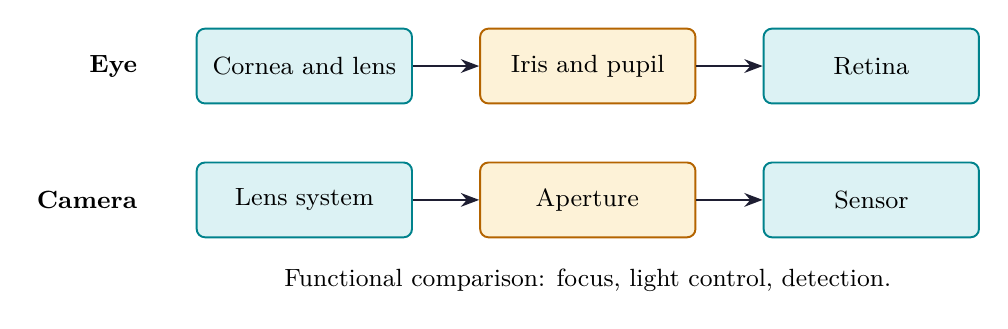
\begin{tikzpicture}[every node/.style={font=\small}]
\foreach \yy/\tag/\focus/\control/\detect in {1.3/Eye/{Cornea and lens}/{Iris and pupil}/{Retina},-0.4/Camera/{Lens system}/{Aperture}/{Sensor}} {
  \node[anchor=east,font=\small\bfseries] at (0,\yy) {\tag};
  \node[block,text width=2.5cm] (a) at (2,\yy) {\focus};
  \node[amberblock,text width=2.5cm] (b) at (5.6,\yy) {\control};
  \node[block,text width=2.5cm] (c) at (9.2,\yy) {\detect};
  \draw[arrow] (a)--(b);
  \draw[arrow] (b)--(c);
}
\node[align=center] at (5.6,-1.42) {Functional comparison: focus, light control, detection.};
\end{tikzpicture}\par
\end{tcolorbox}

\par\vspace{5pt}
\begingroup
\setlength{\extrarowheight}{1pt}
\noindent\begin{tabularx}{\linewidth}{|B{3cm}|Y|Y|}
\hline
\textbf{Function} & \textbf{Human eye} & \textbf{Camera} \\ \hline
Focus & The cornea supplies much of the refraction. Accommodation changes lens shape. & Lens elements focus the image, commonly by moving relative to each other or the sensor. \\ \hline
Control light & The iris changes pupil diameter. Photoreceptors also adapt to light level. & The aperture sets the light opening. Exposure time also controls the collected light. \\ \hline
Detect the image & Rods and cones respond to light. Retinal circuits and the brain process the signals. & Sensor pixels convert light into electrical signals. Electronics record and process the image. \\ \hline
\end{tabularx}\par
\endgroup
\begin{tcolorbox}[masonbox, title={State the limits of the analogy}]
The comparison is functional. The pupil is an opening controlled by the iris. The retina is living neural tissue, while the camera sensor is a manufactured detector. The diagram groups functions rather than showing anatomical order.
\end{tcolorbox}

\subsection{Bird flight and an aircraft}
\begin{itemize}[leftmargin=*, itemsep=3pt, topsep=4pt]
  \item \textbf{Lift.} Bird wings and aircraft wings generate aerodynamic forces as air flows around them. In steady, level, unaccelerated flight, the upward force balances weight.
  \item \textbf{Thrust and drag.} Flapping wings can provide thrust as well as lift. A typical powered fixed-wing aircraft uses a propeller or jet for thrust. In steady level flight, thrust balances drag in the flight direction.
  \item \textbf{Control.} Birds vary wing shape, feathers and tail position. Aircraft may use ailerons, elevators, rudders or other control surfaces.
  \item \textbf{Design lesson.} A natural flyer shows useful principles. An aircraft designer still tests the chosen geometry against load, energy use and stability requirements.
\end{itemize}
\section{How Biological Observations Lead to Discoveries}
\begin{enumerate}[leftmargin=*, itemsep=3pt, topsep=4pt]
  \item \textbf{Observe.} Describe what is seen and under which conditions.
  \item \textbf{Compare.} Deliberately vary a factor or use a comparison case to rule out alternatives.
  \item \textbf{Explain and test.} A proposed cause must predict further outcomes. Later experiments can separate competing explanations.
\end{enumerate}
\begin{tcolorbox}[examplebox, title={An eighteenth-century example: Ingenhousz}]
In 1779, Jan Ingenhousz compared plant effects on air in light and darkness. In sunlight the green portions improved the air by releasing oxygen. Comparing illuminated and shaded material connected the effect to light and green tissues, helping establish a basis for the study of photosynthesis.
\end{tcolorbox}

\begin{tcolorbox}[examplebox, title={Robert Brown and irregular particle motion}]
\begin{itemize}[leftmargin=*, itemsep=3pt, topsep=4pt]
  \item In 1827 Brown observed persistent irregular movement of minute particles suspended in water while examining material from pollen.
  \item He saw similar motion in particles from non-living materials. The comparison showed that the motion did not require living pollen.
  \item The later molecular account explains the random movement as the effect of unequal impacts by moving molecules of the surrounding fluid. Brown recorded the observation in 1828.
\end{itemize}
\end{tcolorbox}

\begin{tcolorbox}[examplebox, title={Julius Robert Mayer and energy conservation}]
\begin{itemize}[leftmargin=*, itemsep=3pt, topsep=4pt]
  \item Mayer noticed unusually bright venous blood while working as a physician in a tropical setting. He considered how different heat demands might affect oxygen use.
  \item The observation inspired a broader question: how are chemical processes, body heat and mechanical work related?
  \item In 1842 he published an early account of the conversion of mechanical work and heat and the conservation of what we now call energy. The observation prompted the idea. Quantitative arguments and experiments were needed to develop the general principle.
\end{itemize}
\end{tcolorbox}

\begin{tcolorbox}[masonbox, title={Exam chronology}]
Use Ingenhousz for the eighteenth century. Brown's observations and Mayer's publication belong to the nineteenth century. The syllabus's Julius Mayor refers to Julius Robert Mayer.
\end{tcolorbox}

\textbf{Primary readings.} \href{https://www.biodiversitylibrary.org/item/127139}{Ingenhousz (1779)}, \href{https://www.rpgroup.caltech.edu/marseillePBoC2024/assets/pdfs/Brown1828.pdf}{Brown (1828)}, and \href{https://web.lemoyne.edu/Giunta/mayer.html}{Mayer (1842, English translation)}.

\subsection{From biological observation to an engineering model}
\begin{tcolorbox}[examplebox, title={Work the eye--camera analogy with a thin lens}]
An object lies $120\,\mathrm{mm}$ in front of a converging camera lens of focal length $24\,\mathrm{mm}$. Use positive distances for this real object and real image.
\[
\begin{aligned}
\frac1v&=\frac1f-\frac1u
=\frac1{24}-\frac1{120}
=\frac1{30}\,\mathrm{mm}^{-1},\\
v&=30\,\mathrm{mm}.
\end{aligned}
\]
For a very distant object, $1/u\approx0$, so the image forms about $24\,\mathrm{mm}$ behind the lens. In the simple camera model, focusing nearer changes the required lens-to-sensor distance. A human eye accommodates by changing lens shape and optical power while the retina's location is approximately fixed.
\end{tcolorbox}

\begin{tcolorbox}[examplebox, title={Turn the flight comparison into a design problem}]
For a $2.0\,\mathrm{kg}$ model aircraft in steady, level flight, assume its wings provide the upward force. Required lift is $L=mg=2.0(9.81)\approx19.6\,\mathrm N$. A bird of the same mass needs the same average vertical support under these conditions. Its moving wings can also generate thrust, so the instantaneous forces vary through a wingbeat. A design team would measure average lift, power and stability separately before choosing a flapping or fixed-wing design.
\end{tcolorbox}

\subsection{What makes an explanation convincing?}
\begin{enumerate}[leftmargin=*, itemsep=2pt]
  \item \textbf{Separate observation and explanation.} Brown observed irregular displacements. Molecular collisions provide a later explanation.
  \item \textbf{Predict a difference.} A steady current would make many nearby particles drift systematically in the same direction. In still fluid, random displacements have no preferred direction.
  \item \textbf{Use repeated observations.} One trajectory can be misleading. Comparing many trajectories helps distinguish a consistent drift from irregular motion.
  \item \textbf{State the limit.} Brown's non-living comparison ruled out a requirement for living particles. Mayer's observation likewise raised an energy question that needed a separate physical argument.
\end{enumerate}

\newpage
\begin{center}
  {\large\bfseries\color{myred} Quick Revision --- Module 1}\\[3pt]
  {\small\color{mydark} Biology and Engineering $|$ BS-B401}
\end{center}
\noindent{\color{myred}\rule{\linewidth}{1.2pt}}\par\vspace{4pt}

\begin{tcolorbox}[formulabox, title={Key Concepts at a Glance}]
\renewcommand{\arraystretch}{1.35}
\noindent\begin{tabularx}{\linewidth}{B{4.5cm}Y}
Science & Explain a natural pattern using testable predictions. \\[3pt]
Engineering & Design and test a solution against requirements. \\[3pt]
Level flight & Lift balances weight and thrust balances drag in steady level flight. \\[3pt]
\end{tabularx}\par
\end{tcolorbox}

\begin{tcolorbox}[defbox, title={One-Line Definitions}]
\begin{itemize}[leftmargin=*, itemsep=3pt, topsep=4pt]
  \item \textbf{Hypothesis.} A testable proposed explanation.
  \item \textbf{Biomimetics.} Engineering inspired by structures or processes in living systems.
  \item \textbf{Brownian motion.} Irregular movement of small suspended particles.
\end{itemize}
\end{tcolorbox}

\begin{tcolorbox}[exambox, title={Frequently Asked / Viva Questions}]
\begin{enumerate}[topsep=0pt, label=\textbf{Q\arabic*.}, itemsep=5pt, leftmargin=*]
  \item \Q{What does biology study?}
    The structure, function, heredity, evolution and interactions of living systems.
  \item \Q{How do scientists test a proposed cause?}
    Compare predictions with measurements and use controls where possible.
  \item \Q{How is an engineering design evaluated?}
    Check its measured performance against the specified requirements.
  \item \Q{What controls pupil diameter?}
    The iris.
  \item \Q{Where is an image detected in the eye?}
    At the retina, where photoreceptors respond to light.
  \item \Q{How can a bird generate thrust?}
    Flapping can push air backwards and generate forward force.
  \item \Q{What did Ingenhousz compare?}
    Plant effects on air in light and darkness.
  \item \Q{How did Brown test whether the motion needed life?}
    He compared material from living sources with non-living particles.
  \item \Q{What question did Mayer's observation prompt?}
    How chemical energy use, heat and work are related.
  \item \Q{When were the three observations reported?}
    Ingenhousz in 1779, Brown in 1828 and Mayer's energy paper in 1842.
\end{enumerate}
\end{tcolorbox}

\begin{tcolorbox}[tikzbox, title={Summary Comparison}]
\par\vspace{5pt}
\begingroup
\setlength{\extrarowheight}{1pt}
\noindent\begin{tabularx}{\linewidth}{|B{3.45cm}|Y|Y|}
\hline
\textbf{Example} & \textbf{Scientific question} & \textbf{Engineering use} \\ \hline
Eye and camera & How does biological vision detect light? & Design focusing, exposure and detection systems. \\ \hline
Bird and aircraft & How do wing motion and shape affect flight? & Design lifting surfaces, propulsion and stability controls. \\ \hline
\end{tabularx}\par
\endgroup
\end{tcolorbox}


% -- Module 2 -----------------------------------------------------------------
\modulestart{2}{Classification and Model Organisms}

\section{Classification and Model Organisms}
\subsection{Levels of organisation and taxonomy}
\begin{tcolorbox}[defbox, title={Classification}]
Classification groups organisms by defined criteria. Taxonomy describes, names and classifies them. Phylogeny concerns their evolutionary relationships. A useful classification states whether the goal is to compare physical traits, ecological roles or common ancestry.
\end{tcolorbox}

\begin{itemize}[leftmargin=*, itemsep=3pt, topsep=4pt]
  \item \textbf{Biological hierarchy.} Molecules form cell components. Cells are the basic units of life. In many multicellular organisms, cells form tissues, organs and organ systems. Individuals form populations, and interacting populations form communities within ecosystems.
  \item \textbf{Taxonomic hierarchy.} Domain, kingdom, phylum, class, order, family, genus and species run from broader to narrower ranked groups. A name such as \textit{Homo sapiens} combines genus and specific epithet.
  \item \textbf{Common thread.} Cells use membranes, genetic information and basic molecular machinery such as ribosomes. Shared inherited features help connect organisms through common descent.
\end{itemize}
\par\vspace{5pt}
\begingroup
\setlength{\extrarowheight}{1pt}
\noindent\begin{tabularx}{\linewidth}{|B{3.2cm}|Y|Y|}
\hline
\textbf{Criterion} & \textbf{Question} & \textbf{Example} \\ \hline
Morphological & What are its observable form and structures? & Body plan or cell shape. \\ \hline
Biochemical & Which compounds and biochemical activities are characteristic? & Membrane lipid types or characteristic metabolic reactions. \\ \hline
Ecological & Where does it live and what ecological role does it fill? & Freshwater producer or soil decomposer. \\ \hline
Molecular & How do homologous molecules compare? & Compare ribosomal RNA sequences to infer relationships. \\ \hline
\end{tabularx}\par
\endgroup
\subsection{Cellularity and ultrastructure}
\par\vspace{5pt}
\begingroup
\setlength{\extrarowheight}{1pt}
\noindent\begin{tabularx}{\linewidth}{|B{3.1cm}|Y|Y|}
\hline
\textbf{Criterion} & \textbf{Categories} & \textbf{Key distinction} \\ \hline
Cellularity & Unicellular or multicellular & A unicellular organism carries out life functions in one cell. Multicellular forms can divide labour among specialised cells. \\ \hline
Nucleus and organelles & Prokaryote or eukaryote & Bacteria and archaea lack a membrane-bound nucleus. Eukaryotes have a nucleus and typically membrane-bound organelles. \\ \hline
Habitat & Aquatic, terrestrial and mixed & Habitat characterises where an organism lives. Some life stages use different environments. \\ \hline
\end{tabularx}\par
\endgroup
\begin{tcolorbox}[masonbox, title={Keep criteria independent}]
Yeast is unicellular and eukaryotic. A multicellular plant is also eukaryotic. The number of cells and presence of a nucleus answer different questions.
\end{tcolorbox}

\subsection{Carbon, energy and electron sources}
\par\vspace{5pt}
\begingroup
\setlength{\extrarowheight}{1pt}
\noindent\begin{tabularx}{\linewidth}{|B{3cm}|Y|Y|}
\hline
\textbf{Dimension} & \textbf{Categories} & \textbf{Meaning} \\ \hline
Carbon & Autotroph or heterotroph & Autotrophs use inorganic carbon such as carbon dioxide. Heterotrophs use preformed organic carbon. \\ \hline
Energy & Phototroph or chemotroph & Phototrophs use light. Chemotrophs obtain energy from chemical reactions. \\ \hline
Electrons & Lithotroph or organotroph & Lithotrophs use inorganic electron donors. Organotrophs use organic donors. \\ \hline
\end{tabularx}\par
\endgroup
\begin{tcolorbox}[examplebox, title={One organism can have several labels}]
An oxygenic green alga is often a photoautotroph because light supplies energy and carbon dioxide supplies carbon. In oxygenic photosynthesis, water is an inorganic electron donor. Humans are chemoorganoheterotrophs because oxidation of organic molecules supplies energy and electrons, and organic molecules supply carbon.
\end{tcolorbox}

\subsection{Nitrogen excretion}
\par\vspace{5pt}
\begingroup
\setlength{\extrarowheight}{1pt}
\noindent\begin{tabularx}{\linewidth}{|B{3.1cm}|Y|Y|}
\hline
\textbf{Group} & \textbf{Main nitrogen product} & \textbf{Typical trade-off and example} \\ \hline
Ammonotelic & Ammonia or ammonium & Highly soluble and toxic. Many aquatic bony fish can eliminate it into surrounding water. \\ \hline
Ureotelic & Urea & Less toxic than ammonia. Synthesis uses energy, but less water is needed for elimination. Example: humans. \\ \hline
Uricotelic & Uric acid & Low solubility helps save water. Production has an energy cost. Example: many birds. \\ \hline
\end{tabularx}\par
\endgroup
\section{Three Domains and Model Organisms}
\subsection{Molecular taxonomy}
\begin{tcolorbox}[defbox, title={Three-domain system}]
Ribosomal RNA comparisons helped distinguish Bacteria, Archaea and Eukarya. A domain is a rank above kingdom. The term Eucarya also appears in the original proposal. This exam framework groups life by evolutionary evidence and does not treat all prokaryotes as one clade.
\end{tcolorbox}

\begin{tcolorbox}[tikzbox, title={The three domain names}]
\centering
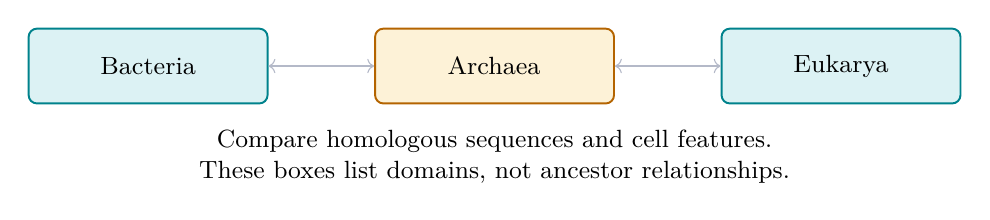
\begin{tikzpicture}[every node/.style={font=\small}]
\node[block,text width=2.8cm] (b) at (0,0) {Bacteria};
\node[amberblock,text width=2.8cm] (a) at (4.4,0) {Archaea};
\node[block,text width=2.8cm] (e) at (8.8,0) {Eukarya};
\draw[mgframe,<->] (b.east)--(a.west);
\draw[mgframe,<->] (a.east)--(e.west);
\node[align=center] at (4.4,-1.15) {Compare homologous sequences and cell features.\\These boxes list domains, not ancestor relationships.};
\end{tikzpicture}\par
\end{tcolorbox}

\textbf{Primary reading.} \href{https://pubmed.ncbi.nlm.nih.gov/2112744/}{Woese, Kandler and Wheelis (1990), three-domain proposal}.
\subsection{Six syllabus model organisms}
\par\vspace{5pt}
\begingroup
\setlength{\extrarowheight}{1pt}
\noindent\begin{tabularx}{\linewidth}{|B{4.2cm}|Y|Y|}
\hline
\textbf{Organism} & \textbf{Group} & \textbf{Why it is studied} \\ \hline
\textit{Escherichia coli} & Bacterium & Basic cell physiology and gene regulation, using well-characterised teaching and research strains. \\ \hline
\textit{Saccharomyces cerevisiae} & Budding yeast, unicellular fungus & Eukaryotic cell cycle, metabolism and genetics. \\ \hline
\textit{Drosophila melanogaster} & Fruit fly, animal & Inheritance, chromosome linkage and development. \\ \hline
\textit{Caenorhabditis elegans} & Nematode, animal & Cell lineage, development and programmed cell death. \\ \hline
\textit{Arabidopsis thaliana} & Flowering plant & Plant development, signalling and genetics. \\ \hline
\textit{Mus musculus} & House mouse, mammal & Mammalian physiology, development and inheritance. \\ \hline
\end{tabularx}\par
\endgroup
\begin{tcolorbox}[examplebox, title={Choose a model for a question}]
A researcher asking how a plant responds to light can use Arabidopsis. A question about a mammalian organ requires a different model. Model choice depends on the feature studied, available measurements and how far conclusions can be transferred.
\end{tcolorbox}

\subsection{How to classify when observable traits disagree}
\begin{enumerate}[leftmargin=*, itemsep=2pt]
  \item \textbf{Define the question.} A habitat group answers an ecological question. A group based on descent answers an evolutionary one.
  \item \textbf{Distinguish homology and convergence.} Homologous features are inherited from a common ancestor. Similar shapes can also evolve independently under similar pressures.
  \item \textbf{Use more than one kind of evidence.} Combine morphology and cellular features with comparable molecular characters. Different lines of evidence may test the same proposed relationship.
  \item \textbf{Read the branch point.} If two groups share a more recent branch point with each other than with a third group, they are closer relatives on that tree. The spacing of their names on the page is irrelevant.
\end{enumerate}

\begin{tcolorbox}[examplebox, title={Compare a whale, a fish and a land mammal}]
A whale and a fish share an aquatic habitat and a streamlined shape. A whale and a land mammal share mammalian characteristics and a more recent common ancestor. The first grouping answers where the animals live, whereas the second answers how they are related. State the criterion before defending a classification.
\end{tcolorbox}

\subsection{Explain nitrogen excretion as a water and energy trade-off}
\begin{itemize}[leftmargin=*, itemsep=2pt]
  \item \textbf{Ammonia.} Direct elimination can work where plentiful surrounding water carries soluble waste away.
  \item \textbf{Urea.} Converting nitrogen into urea costs energy, but its lower toxicity permits more concentrated elimination.
  \item \textbf{Uric acid.} Low solubility can conserve water. It also permits nitrogenous waste to accumulate in a relatively insoluble form within a shelled egg.
  \item \textbf{Qualification.} The category identifies the main excretion product under the conditions studied. The balance can change with life stage or environment.
\end{itemize}

\begin{tcolorbox}[masonbox, title={Defend a choice of model organism}]
Select a yeast for a basic eukaryotic cell-cycle question, the fruit fly or nematode for many developmental questions, Arabidopsis for plant traits, and the mouse for mammalian physiology. A shared cell mechanism can be informative across species. Whole-organism conclusions still depend on the tissue, trait and biological context.
\end{tcolorbox}

\newpage
\begin{center}
  {\large\bfseries\color{myred} Quick Revision --- Module 2}\\[3pt]
  {\small\color{mydark} Classification and Model Organisms $|$ BS-B401}
\end{center}
\noindent{\color{myred}\rule{\linewidth}{1.2pt}}\par\vspace{4pt}

\begin{tcolorbox}[formulabox, title={Key Concepts at a Glance}]
\renewcommand{\arraystretch}{1.35}
\noindent\begin{tabularx}{\linewidth}{B{4.5cm}Y}
Cell structure & Bacteria and Archaea are prokaryotic. Eukarya have a nucleus. \\[3pt]
Nutritional axes & Carbon, energy and electron source are independent dimensions. \\[3pt]
Taxonomy & Molecular comparisons add ancestry evidence to physical and ecological traits. \\[3pt]
\end{tabularx}\par
\end{tcolorbox}

\begin{tcolorbox}[defbox, title={One-Line Definitions}]
\begin{itemize}[leftmargin=*, itemsep=3pt, topsep=4pt]
  \item \textbf{Taxon.} A named group at any taxonomic rank.
  \item \textbf{Autotroph.} Organism that uses inorganic carbon as its principal carbon source.
  \item \textbf{Lithotroph.} Organism using inorganic electron donors.
\end{itemize}
\end{tcolorbox}

\begin{tcolorbox}[exambox, title={Frequently Asked / Viva Questions}]
\begin{enumerate}[topsep=0pt, label=\textbf{Q\arabic*.}, itemsep=5pt, leftmargin=*]
  \item \Q{What is the basic unit of life?}
    The cell.
  \item \Q{How does phylogeny differ from taxonomy?}
    Phylogeny deals with evolutionary relationships. Taxonomy names and classifies groups.
  \item \Q{Is every unicellular organism prokaryotic?}
    Yeast is a unicellular eukaryote.
  \item \Q{What are the three domains?}
    Bacteria, Archaea and Eukarya.
  \item \Q{Why use ribosomal RNA for comparisons?}
    Related ribosomal genes are widely shared and contain both conserved and variable features.
  \item \Q{Is lithotrophy a carbon label?}
    It describes electron donors.
  \item \Q{Which excretory product helps conserve water?}
    Uric acid.
  \item \Q{Name a plant model.}
    Arabidopsis thaliana.
  \item \Q{Name a unicellular eukaryotic model.}
    Saccharomyces cerevisiae.
  \item \Q{Why can an organism belong to several categories?}
    Each criterion describes a different feature.
\end{enumerate}
\end{tcolorbox}

\begin{tcolorbox}[tikzbox, title={Summary Comparison}]
\par\vspace{5pt}
\begingroup
\setlength{\extrarowheight}{1pt}
\noindent\begin{tabularx}{\linewidth}{|B{3.45cm}|Y|Y|}
\hline
\textbf{Criterion} & \textbf{One label} & \textbf{A distinct feature} \\ \hline
Carbon & Autotroph & Source of cell carbon. \\ \hline
Electrons & Lithotroph & Origin of electrons used in metabolism. \\ \hline
Nitrogen excretion & Ureotelic & Principal nitrogenous waste. \\ \hline
\end{tabularx}\par
\endgroup
\end{tcolorbox}


% -- Module 3 -----------------------------------------------------------------
\modulestart{3}{Genetics}

\section{Genetics}
\subsection{Gene, allele and trait}
\begin{tcolorbox}[defbox, title={Foundations of heredity}]
A gene is a unit of heredity associated with a functional product. An allele is a variant of a gene at a particular locus, or chromosome position. Genotype is the genetic constitution being described. Phenotype is the observable trait and can depend on genotype, environment and development.
\end{tcolorbox}

\begin{itemize}[leftmargin=*, itemsep=3pt, topsep=4pt]
  \item \textbf{Diploid inheritance.} Two homologous chromosomes usually carry the same loci, one inherited from each parent. A homozygote has the same allele at a locus. A heterozygote has different alleles there.
  \item \textbf{Dominance.} With complete dominance, the heterozygote has the same scored phenotype as one homozygote. The other allele is recessive for that phenotype. Dominance says nothing about population frequency or fitness.
  \item \textbf{Other relationships.} In incomplete dominance the heterozygote is intermediate. In codominance both allele products are distinguishable, as with the A and B antigens of the human ABO blood group.
\end{itemize}
\subsection{Mendel's laws and predictions}
\begin{enumerate}[leftmargin=*, itemsep=3pt, topsep=4pt]
  \item \textbf{Segregation.} The two alleles at a locus separate during gamete formation. For a simple $Aa$ parent, each type of gamete normally carries one allele, with probabilities $1/2$ each.
  \item \textbf{Independent assortment.} Allele pairs at different unlinked loci assort independently. An $AaBb$ parent makes $AB$, $Ab$, $aB$ and $ab$ gametes in equal proportions under this condition.
  \item \textbf{Fertilisation.} One gamete from each parent combines to restore the diploid number. Multiply independent probabilities and add probabilities of mutually exclusive paths to the same outcome.
\end{enumerate}
\begin{tcolorbox}[examplebox, title={Monohybrid and dihybrid crosses}]
\par\vspace{5pt}
\begingroup
\setlength{\extrarowheight}{1pt}
\noindent\begin{tabularx}{\linewidth}{|B{3.5cm}|Y|Y|}
\hline
\textbf{Cross} & \textbf{Genotypes or gametes} & \textbf{Phenotypes under complete dominance} \\ \hline
$Aa\times Aa$ & $AA:Aa:aa=1:2:1$. The two routes to $Aa$ each contribute $1/4$. & Dominant to recessive $=3:1$. \\ \hline
$AaBb\times AaBb$ & Each parent makes four equally likely gametes if the loci are unlinked. & $A\_B\_:A\_bb:aaB\_:aabb=9:3:3:1$. \\ \hline
$Aa\times aa$ & Progeny $Aa:aa=1:1$. & A testcross uses the recessive homozygote to reveal the alleles in the other parent's gametes. \\ \hline
\end{tabularx}\par
\endgroup
For the dihybrid cross, $P(A\_B\_)=(3/4)(3/4)=9/16$ and $P(aabb)=(1/4)(1/4)=1/16$. Here an underscore means either allele in that position. The prediction assumes independent assortment, complete dominance and no viability differences.
\end{tcolorbox}

\subsection{What mitosis and meiosis transmit}
\begin{tcolorbox}[tikzbox, title={Genetic transmission across generations}]
\centering
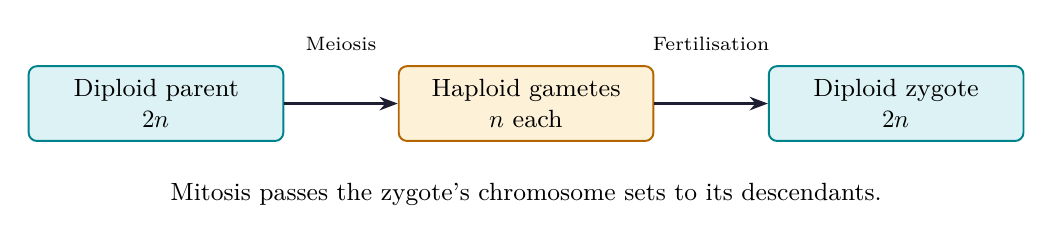
\begin{tikzpicture}[every node/.style={font=\small}]
\node[block,text width=3cm] (p) at (0,0) {Diploid parent\\$2n$};
\node[amberblock,text width=3cm] (g) at (4.7,0) {Haploid gametes\\$n$ each};
\node[block,text width=3cm] (z) at (9.4,0) {Diploid zygote\\$2n$};
\draw[arrow] (p)--(g);
\draw[arrow] (g)--(z);
\node[font=\scriptsize] at (2.35,0.76) {Meiosis};
\node[font=\scriptsize] at (7.05,0.76) {Fertilisation};
\node at (4.7,-1.15) {Mitosis passes the zygote's chromosome sets to its descendants.};
\end{tikzpicture}\par
\end{tcolorbox}

\par\vspace{5pt}
\begingroup
\setlength{\extrarowheight}{1pt}
\noindent\begin{tabularx}{\linewidth}{|B{3cm}|Y|Y|}
\hline
\textbf{Feature} & \textbf{Mitosis} & \textbf{Meiosis} \\ \hline
Primary role & Growth, maintenance and asexual cell proliferation. & Form haploid cells for sexual reproduction or for a haploid life stage. \\ \hline
Chromosome sets & Preserves ploidy in ordinary division. & One replication followed by two divisions reduces diploid to haploid. \\ \hline
What separates & Sister chromatids separate. & Homologues separate first. Sister chromatids then separate. \\ \hline
Diversity & Daughter cells are usually genetically similar. & Independent orientation and crossing over can produce new allele combinations. \\ \hline
\end{tabularx}\par
\endgroup
\section{Linkage, Gene Interaction and Human Inheritance}
\subsection{Linkage and gene mapping}
Linked loci on the same chromosome can be inherited together more often than predicted by independent assortment. Crossing over between homologous chromosomes creates recombinant combinations.
\begin{tcolorbox}[examplebox, title={Map two loci using a testcross}]
A heterozygote $AB/ab$ is crossed with $ab/ab$. The counts for $AB,ab,Ab,aB$ gametes are 420, 420, 80 and 80. The rare types are recombinant.
\[
\text{Recombination fraction}=\frac{80+80}{1000}=0.16.
\]
A short-interval estimate is about 16 map units (centimorgans). A two-point recombination fraction approaches at most 50\% even when multiple crossovers occur, so it may underestimate large map distances.
\end{tcolorbox}

\subsection{Gene interaction and epistasis}
\begin{tcolorbox}[defbox, title={Epistasis}]
Epistasis occurs when genotype at one locus changes or masks the phenotype expected at another locus. Dominance compares alleles at a single locus.
\end{tcolorbox}

\begin{tcolorbox}[examplebox, title={How recessive epistasis changes a ratio}]
Suppose $E$ permits pigment deposition and $ee$ prevents it. Among animals that can deposit pigment, $B\_$ gives dark colour and $bb$ gives brown colour. From a dihybrid cross, $9/16$ are $B\_E\_$, $3/16$ are $bbE\_$ and $4/16$ are $\_\_ee$. The phenotype ratio is $9:3:4$ because the two $ee$ classes look alike.
\end{tcolorbox}

\subsection{From phenotype to gene and complementation}
\begin{enumerate}[leftmargin=*, itemsep=3pt, topsep=4pt]
  \item \textbf{Record the phenotype.} Decide what is being scored and record variation and family relationships.
  \item \textbf{Infer a model.} Use segregation and pedigrees to predict dominant, recessive or other possible inheritance patterns.
  \item \textbf{Test the locus.} Ask whether the trait and nearby markers are inherited together. Recombination can narrow an interval. Independent functional evidence helps distinguish a causal gene from its neighbours.
\end{enumerate}
\par\vspace{5pt}
\begingroup
\setlength{\extrarowheight}{1pt}
\noindent\begin{tabularx}{\linewidth}{|B{3.2cm}|Y|Y|}
\hline
\textbf{Single-gene example} & \textbf{Inheritance typically taught} & \textbf{Biological link} \\ \hline
Cystic fibrosis & Autosomal recessive. & Pathogenic variants in \textit{CFTR} affect ion transport. \\ \hline
Sickle cell disease & Autosomal recessive inheritance for the HbSS example. & Variants of \textit{HBB} change beta-globin. Other allele combinations can also cause disease. \\ \hline
Huntington disease & Autosomal dominant. & An expanded repeat in \textit{HTT} contributes to progressive neurological disease. \\ \hline
\end{tabularx}\par
\endgroup
\begin{tcolorbox}[examplebox, title={Human genetics thought experiment: complementation}]
Two unrelated parents have similar recessive hearing phenotypes. Assume one is $aaBB$ and the other $AAbb$, and that a functional copy of both genes is needed for typical hearing. A child $AaBb$ has a functional copy at each locus and is predicted to complement. If the parents instead both have the same recessive cause, represented here as $aa$, their children would lack a functional $A$ allele. This simplified model explains why apparently similar phenotypes can involve different genes.
\end{tcolorbox}

\begin{tcolorbox}[masonbox, title={Use the assumptions}]
Complementation is interpreted for recessive variants under an appropriate loss-of-function model. Real pedigrees may also reflect penetrance, environment or more than one contributing locus.
\end{tcolorbox}

\textbf{Primary reading.} \href{https://doi.org/10.1534/genetics.116.195198}{Mendel's 1866 paper in English translation}.

\subsection{Build a Mendelian answer from the gametes}
\begin{tcolorbox}[examplebox, title={Read a Punnett square and account for each outcome}]
For $Aa\times Aa$, each parent contributes $A$ or $a$ with probability $1/2$. Each square has probability $1/4$.
\par\vspace{6pt}
\noindent\begin{tabularx}{\linewidth}{|B{3.5cm}|Y|Y|}
\hline
\textbf{Gamete from the first parent} & \textbf{$A$ from the second} & \textbf{$a$ from the second} \\ \hline
$A$ & $AA$ & $Aa$ \\ \hline
$a$ & $Aa$ & $aa$ \\ \hline
\end{tabularx}\par\smallskip

So $P(AA)=1/4$, $P(Aa)=1/2$, and $P(aa)=1/4$. With complete dominance, $AA$ and $Aa$ join in one phenotype class, giving $3:1$ while the genotype ratio remains $1:2:1$. Random inheritance can produce different counts in a small family.
\end{tcolorbox}

\subsection{Reason from a pedigree}
\begin{enumerate}[leftmargin=*, itemsep=2pt]
  \item \textbf{Propose a model.} Two unaffected parents have an affected child. Under the simple autosomal recessive model with complete penetrance, both parents can be $Aa$ carriers and the affected child is $aa$.
  \item \textbf{Predict a new outcome.} The probability of an affected child in another pregnancy is $1/4$ under that model.
  \item \textbf{Use conditional probability when needed.} If a child is known to be unaffected, exclude the $aa$ square. Two of the three equally likely remaining squares are $Aa$, giving carrier probability $2/3$.
  \item \textbf{Check the assumptions.} One short pedigree may fit several models. Other relatives, marker inheritance or functional evidence help distinguish them.
\end{enumerate}

\subsection{Why linkage and epistasis change different results}
\begin{itemize}[leftmargin=*, itemsep=2pt]
  \item \textbf{Linkage changes gamete frequencies.} A testcross may reveal two abundant parental combinations. Count both recombinant classes before using the recombination fraction.
  \item \textbf{Epistasis changes the phenotype grouping.} For the pigment example, $B\_ee$ contributes $3/16$ and $bbee$ contributes $1/16$. Both lack pigment deposition, so the two form one $4/16$ class. The two loci can still assort independently.
  \item \textbf{Complementation helps distinguish loci.} Two recessive defects may look similar because the affected genes contribute to the same task. Under the stated assumptions the offspring restores that task by inheriting a functional copy at each locus.
\end{itemize}

\newpage
\begin{center}
  {\large\bfseries\color{myred} Quick Revision --- Module 3}\\[3pt]
  {\small\color{mydark} Genetics $|$ BS-B401}
\end{center}
\noindent{\color{myred}\rule{\linewidth}{1.2pt}}\par\vspace{4pt}

\begin{tcolorbox}[formulabox, title={Key Concepts at a Glance}]
\renewcommand{\arraystretch}{1.35}
\noindent\begin{tabularx}{\linewidth}{B{4.5cm}Y}
Monohybrid cross & $Aa\times Aa$: genotype $1:2:1$ and, with complete dominance, phenotype $3:1$. \\[3pt]
Independent events & Multiply probabilities for independent gamete outcomes. \\[3pt]
Map distance & Recombinants divided by total progeny, converted to percentage for a short interval. \\[3pt]
\end{tabularx}\par
\end{tcolorbox}

\begin{tcolorbox}[defbox, title={One-Line Definitions}]
\begin{itemize}[leftmargin=*, itemsep=3pt, topsep=4pt]
  \item \textbf{Allele.} A variant at a genetic locus.
  \item \textbf{Epistasis.} Interaction in which one locus alters the phenotypic effect of another.
  \item \textbf{Complementation.} Restoration of function by combining variants that leave functional copies at different loci.
\end{itemize}
\end{tcolorbox}

\begin{tcolorbox}[exambox, title={Frequently Asked / Viva Questions}]
\begin{enumerate}[topsep=0pt, label=\textbf{Q\arabic*.}, itemsep=5pt, leftmargin=*]
  \item \Q{What segregates during gamete formation?}
    The two alleles at a locus.
  \item \Q{When is independent assortment a good prediction?}
    For unlinked loci, or loci effectively unlinked in the observed cross.
  \item \Q{What is a testcross?}
    A cross to a recessive homozygote to reveal gamete types.
  \item \Q{Does dominance mean commonness?}
    Dominance describes the phenotype of a heterozygote.
  \item \Q{Which division reduces ploidy?}
    Meiosis.
  \item \Q{Why can linked loci produce recombinants?}
    Crossing over can exchange material between homologues.
  \item \Q{What is a centimorgan?}
    A genetic map unit, approximated by one percent recombination over a short interval.
  \item \Q{Why can epistasis produce 9:3:4?}
    Two genotype categories merge because one genotype masks the other locus.
  \item \Q{What does a pedigree show?}
    Trait transmission across relatives and generations.
  \item \Q{What does two-locus complementation indicate under the simple model?}
    Each parent carries a different recessive cause. A functional copy at each locus restores the trait.
\end{enumerate}
\end{tcolorbox}

\begin{tcolorbox}[tikzbox, title={Summary Comparison}]
\par\vspace{5pt}
\begingroup
\setlength{\extrarowheight}{1pt}
\noindent\begin{tabularx}{\linewidth}{|B{3.45cm}|Y|Y|}
\hline
\textbf{Concept} & \textbf{Scale} & \textbf{Typical clue} \\ \hline
Dominance & One locus & Phenotype of a heterozygote. \\ \hline
Epistasis & Two or more loci & One locus masks or modifies another. \\ \hline
Linkage & Chromosome region & Parental gamete classes occur in excess. \\ \hline
\end{tabularx}\par
\endgroup
\end{tcolorbox}


% -- Module 4 -----------------------------------------------------------------
\modulestart{4}{Biomolecules}

\section{Biomolecules}
\subsection{Shared building blocks and different structures}
\begin{tcolorbox}[defbox, title={Monomer and polymer}]
A monomer is a small building unit that can be joined to others. A polymer contains repeated or related units connected by covalent bonds. The arrangement, linkage and branching of its building blocks influence function. Most lipids are assembled molecules rather than repeating-chain polymers.
\end{tcolorbox}

\par\vspace{5pt}
\begingroup
\setlength{\extrarowheight}{1pt}
\noindent\begin{tabularx}{\linewidth}{|B{3.1cm}|Y|Y|}
\hline
\textbf{Family} & \textbf{Units and linkage} & \textbf{Biological roles} \\ \hline
Carbohydrates & Monosaccharides joined by glycosidic bonds. & Fuel, storage, recognition and structural support. \\ \hline
Proteins & Amino acids joined by peptide bonds. & Catalysis, transport, signalling and structure. \\ \hline
Nucleic acids & Nucleotides joined by phosphodiester bonds. & Information storage, transfer and some catalysis. \\ \hline
Lipids & Fatty acids, glycerol or other lipid precursors assembled into different families. & Energy storage, membranes and signalling. \\ \hline
\end{tabularx}\par
\endgroup
\subsection{Sugars, starch and cellulose}
\begin{itemize}[leftmargin=*, itemsep=3pt, topsep=4pt]
  \item \textbf{Monosaccharide.} A single sugar unit, such as glucose, ribose or fructose. Glucose is a common metabolic fuel. Ribose is a component of RNA.
  \item \textbf{Disaccharide.} Two sugar units linked by a glycosidic bond. Sucrose contains glucose and fructose.
  \item \textbf{Configuration.} The $\alpha$ and $\beta$ labels distinguish stereochemistry at the anomeric carbon. This difference changes the direction in which glucose units link.
\end{itemize}
\par\vspace{5pt}
\begingroup
\setlength{\extrarowheight}{1pt}
\noindent\begin{tabularx}{\linewidth}{|B{3.1cm}|Y|Y|}
\hline
\textbf{Polysaccharide} & \textbf{Linkages and shape} & \textbf{Function} \\ \hline
Starch: amylose & Mostly linear $\alpha(1\to4)$ glucose chains. Chains can coil. & Plant storage carbohydrate. \\ \hline
Starch: amylopectin & $\alpha(1\to4)$ main chains with $\alpha(1\to6)$ branch points. & Branched component of plant starch. \\ \hline
Cellulose & Linear $\beta(1\to4)$ glucose chains. Adjacent chains associate through hydrogen bonding. & Tough plant cell-wall microfibrils. \\ \hline
\end{tabularx}\par
\endgroup
\begin{tcolorbox}[examplebox, title={Same monomer, different material}]
Starch and cellulose both contain glucose. Human digestive enzymes can hydrolyse the common starch linkages, while humans lack cellulase for the cellulose linkage. The different bond geometry also helps cellulose form extended fibres, making it suitable for support.
\end{tcolorbox}

\subsection{Amino acids and proteins}
An ordinary alpha-amino acid has an alpha carbon attached to an amino group, a carboxyl group, a hydrogen and a side chain $R$. Glycine has $R=\mathrm H$. The side chain affects polarity, charge and interactions.
\begin{enumerate}[leftmargin=*, itemsep=3pt, topsep=4pt]
  \item \textbf{Join.} A peptide bond joins the carboxyl-derived carbon of one residue to the amino-derived nitrogen of the next. In a simplified chemical representation, joining releases water.
  \item \textbf{Read direction.} A protein sequence is conventionally written from the amino (N) terminus to the carboxyl (C) terminus.
  \item \textbf{Fold.} The order and interactions of side chains influence a polypeptide's shape. The resulting structure contributes to function. Module 7 develops the four levels of organisation.
\end{enumerate}
\subsection{Nucleotides and nucleic acids}
\begin{tcolorbox}[defbox, title={Nucleotide}]
A nucleotide contains a nitrogenous base, a pentose sugar and at least one phosphate group. A nucleoside is a base plus sugar. In DNA and RNA, phosphodiester linkages connect the sugars through phosphate groups to form a directional backbone.
\end{tcolorbox}

\par\vspace{5pt}
\begingroup
\setlength{\extrarowheight}{1pt}
\noindent\begin{tabularx}{\linewidth}{|B{3.1cm}|Y|Y|}
\hline
\textbf{Property} & \textbf{DNA} & \textbf{RNA} \\ \hline
Sugar & Deoxyribose. & Ribose. \\ \hline
Bases & A, T, G and C. & A, U, G and C. \\ \hline
Common organisation & Double-stranded helix in cells. & Often single-stranded, with complementary regions folded into local structures. \\ \hline
Typical roles & Stable cellular hereditary information. & Messages, adaptors, structural and catalytic roles. \\ \hline
\end{tabularx}\par
\endgroup
\section{Lipids and the Two-Carbon Unit}
\subsection{Acetyl units, fatty acids and lipid classes}
\begin{itemize}[leftmargin=*, itemsep=3pt, topsep=4pt]
  \item \textbf{Acetyl unit.} Acetyl-CoA carries a two-carbon acetyl group and links carbohydrate, fatty acid and amino acid metabolism.
  \item \textbf{Chain growth.} In fatty-acid synthesis, acetyl-derived building blocks supply two-carbon additions. Malonyl groups provide the elongating units after loss of carbon dioxide.
  \item \textbf{Chain breakdown.} Beta-oxidation shortens many fatty acids, releasing two-carbon acetyl-CoA units.
  \item \textbf{Packing.} Saturated chains have no carbon--carbon double bonds. A cis double bond can kink an unsaturated chain and reduce tight packing. Amphipathic phospholipids organise into bilayers in water.
\end{itemize}
\par\vspace{5pt}
\begingroup
\setlength{\extrarowheight}{1pt}
\noindent\begin{tabularx}{\linewidth}{|B{3.2cm}|Y|Y|}
\hline
\textbf{Lipid class} & \textbf{Structure to recognise} & \textbf{Role} \\ \hline
Triacylglycerol & Three fatty acids esterified to glycerol. & Energy storage. \\ \hline
Phospholipid & A polar phosphate-containing head and hydrophobic regions. & Amphipathic membrane component. \\ \hline
Sterol & A rigid fused-ring structure with a small polar part. & Cholesterol contributes to animal membranes and is a precursor for other compounds. \\ \hline
\end{tabularx}\par
\endgroup
\begin{tcolorbox}[tikzbox, title={Simplified phospholipid bilayer}]
\centering
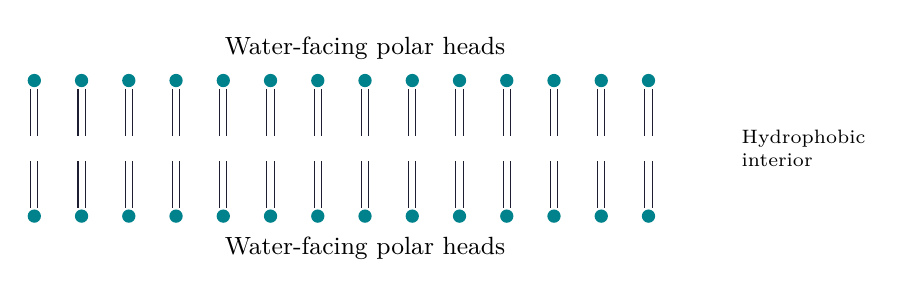
\begin{tikzpicture}[y=0.82cm,every node/.style={font=\small}]
\foreach \x in {0,0.6,...,8.4}{
  \fill[myteal] (\x,1.05) circle (2.4pt);
  \fill[myteal] (\x,-1.05) circle (2.4pt);
  \draw[mydark] ([xshift=-1.3pt]\x,0.92)--([xshift=-1.3pt]\x,0.19)
                 ([xshift=1.3pt]\x,0.92)--([xshift=1.3pt]\x,0.19);
  \draw[mydark] ([xshift=-1.3pt]\x,-0.92)--([xshift=-1.3pt]\x,-0.19)
                 ([xshift=1.3pt]\x,-0.92)--([xshift=1.3pt]\x,-0.19);
}
\node[font=\small] at (4.2,1.55) {Water-facing polar heads};
\node[font=\small] at (4.2,-1.55) {Water-facing polar heads};
\node[anchor=west,align=left,font=\scriptsize] at (8.86,0) {Hydrophobic\\interior};
\end{tikzpicture}\par
\end{tcolorbox}



\subsection{Relate bond chemistry to macromolecular behaviour}
\par\vspace{6pt}
\noindent\begin{tabularx}{\linewidth}{|B{3.2cm}|Y|Y|}
\hline
\textbf{Bond or interaction} & \textbf{Where it matters} & \textbf{Consequence} \\ \hline
Glycosidic bond & Links sugar residues at specified carbon positions. & Changing the linkage can change shape and which enzymes recognise the chain. \\ \hline
Peptide bond & Links the carboxyl-derived carbon of one residue to the amino-derived nitrogen of the next. & Gives a directional polypeptide backbone. \\ \hline
Phosphodiester bond & Joins neighbouring sugars through a phosphate. & Creates a directional, negatively charged nucleic-acid backbone. \\ \hline
Hydrogen bonding & Between cellulose chains, or between complementary bases in DNA. & Helps stabilise a structure without being the covalent linkage along either chain. \\ \hline
\end{tabularx}\par

\begin{tcolorbox}[examplebox, title={Explain reducing and nonreducing sugars}]
A reducing sugar has an anomeric centre that can open to a form with a reactive carbonyl group. In maltose, one anomeric carbon remains free. In sucrose, the glycosidic linkage joins the anomeric carbons of glucose and fructose, leaving neither free. This structural distinction explains why the two disaccharides can behave differently even though both contain two sugar units.
\end{tcolorbox}

\subsection{Use chain direction and unit count correctly}
\begin{itemize}[leftmargin=*, itemsep=2pt]
  \item \textbf{Polypeptide.} A single unbranched chain with $n$ amino-acid residues has $n-1$ peptide bonds. A chain of eight residues therefore has seven such bonds and one N terminus and one C terminus.
  \item \textbf{Nucleic acid.} A single linear strand with $n$ nucleotides contains $n-1$ internucleotide phosphodiester linkages. The two strands of a DNA duplex each have their own backbone.
  \item \textbf{Fat.} A triacylglycerol uses three ester bonds to attach three fatty acids to one glycerol. Its architecture is an assembly around glycerol rather than a long chain of identical lipid monomers.
\end{itemize}

\begin{tcolorbox}[masonbox, title={Explain why bilayers are selective}]
Water and ions interact differently with the hydrophobic interior. Charged solutes cross an intact lipid region poorly and often need transport proteins. This links amphipathic structure in this module to selective transport in Module 7.
\end{tcolorbox}

\newpage
\begin{center}
  {\large\bfseries\color{myred} Quick Revision --- Module 4}\\[3pt]
  {\small\color{mydark} Biomolecules $|$ BS-B401}
\end{center}
\noindent{\color{myred}\rule{\linewidth}{1.2pt}}\par\vspace{4pt}

\begin{tcolorbox}[formulabox, title={Key Concepts at a Glance}]
\renewcommand{\arraystretch}{1.35}
\noindent\begin{tabularx}{\linewidth}{B{4.5cm}Y}
Carbohydrate bond & Glycosidic bonds connect sugar units. \\[3pt]
Protein bond & Peptide bonds connect amino-acid residues. \\[3pt]
Nucleic acid backbone & Phosphodiester bonds connect nucleotides in a directional chain. \\[3pt]
Acetyl-CoA & Carries a two-carbon acetyl group. \\[3pt]
\end{tabularx}\par
\end{tcolorbox}

\begin{tcolorbox}[defbox, title={One-Line Definitions}]
\begin{itemize}[leftmargin=*, itemsep=3pt, topsep=4pt]
  \item \textbf{Polysaccharide.} Polymer of monosaccharides.
  \item \textbf{Nucleoside.} A base and sugar without the phosphate group.
  \item \textbf{Amphipathic.} Having both hydrophilic and hydrophobic regions.
\end{itemize}
\end{tcolorbox}

\begin{tcolorbox}[exambox, title={Frequently Asked / Viva Questions}]
\begin{enumerate}[topsep=0pt, label=\textbf{Q\arabic*.}, itemsep=5pt, leftmargin=*]
  \item \Q{What controls polymer function?}
    The identity, arrangement and connectivity of its units.
  \item \Q{What is the major monomer in starch and cellulose?}
    Glucose.
  \item \Q{Which linkage forms cellulose?}
    $\beta(1\to4)$ between glucose residues.
  \item \Q{What creates branches in amylopectin?}
    $\alpha(1\to6)$ linkages.
  \item \Q{What is a peptide bond?}
    The amide linkage joining adjacent amino-acid residues.
  \item \Q{What distinguishes a nucleotide from a nucleoside?}
    A nucleotide has phosphate in addition to base and sugar.
  \item \Q{Which sugar is present in RNA?}
    Ribose.
  \item \Q{What molecule carries a two-carbon acetyl unit?}
    Acetyl-CoA.
  \item \Q{How many fatty acids are present in a triacylglycerol?}
    Three, esterified to glycerol.
  \item \Q{Why do phospholipids form bilayers?}
    Water-compatible heads face water and hydrophobic parts associate in the interior.
\end{enumerate}
\end{tcolorbox}

\begin{tcolorbox}[tikzbox, title={Summary Comparison}]
\par\vspace{5pt}
\begingroup
\setlength{\extrarowheight}{1pt}
\noindent\begin{tabularx}{\linewidth}{|B{3.45cm}|Y|Y|}
\hline
\textbf{Molecule} & \textbf{Building unit} & \textbf{Typical role} \\ \hline
Starch & Glucose & Plant storage. \\ \hline
Cellulose & Glucose & Plant structural fibres. \\ \hline
Protein & Amino acids & Many cellular functions. \\ \hline
DNA & Deoxyribonucleotides & Hereditary information. \\ \hline
\end{tabularx}\par
\endgroup
\end{tcolorbox}


% -- Module 5 -----------------------------------------------------------------
\modulestart{5}{Enzymes}

\section{Enzymes}
\subsection{Catalysis and the active site}
\begin{tcolorbox}[defbox, title={Enzyme}]
An enzyme is a biological catalyst. It increases the rate at which a reaction approaches equilibrium by lowering the activation free-energy barrier. It does not change the reaction's overall free-energy difference or equilibrium constant. Most enzymes are proteins. Some RNAs also catalyse reactions.
\end{tcolorbox}

\begin{enumerate}[leftmargin=*, itemsep=3pt, topsep=4pt]
  \item \textbf{Bind.} Substrate binds in an active site through multiple interactions. In induced fit, binding shifts the conformations of enzyme and substrate.
  \item \textbf{Catalyse.} The site can orient reactants, stabilise the transition state, transfer protons, use a metal ion, or form a short-lived covalent intermediate.
  \item \textbf{Release.} Product leaves and the enzyme can act again. Binding the substrate very tightly alone does not guarantee rapid catalysis.
\end{enumerate}
\begin{tcolorbox}[examplebox, title={Two mechanisms with different chemical roles}]
\begin{itemize}[leftmargin=*, itemsep=3pt, topsep=4pt]
  \item \textbf{Lactase: hydrolysis.} It breaks the glycosidic bond in lactose to give glucose and galactose. Catalytic groups help transfer protons during cleavage. Water supplies the elements added across the broken bond.
  \item \textbf{Carbonic anhydrase: metal-assisted catalysis.} It accelerates reversible conversion of carbon dioxide and water into bicarbonate and a proton. A zinc ion helps activate bound water. The resulting hydroxide attacks carbon dioxide, followed by product release and regeneration of the active site.
\end{itemize}
\end{tcolorbox}

\subsection{Classification by reaction type}
\par\vspace{5pt}
\begingroup
\setlength{\extrarowheight}{1pt}
\noindent\begin{tabularx}{\linewidth}{|B{3.5cm}|Y|Y|}
\hline
\textbf{Class} & \textbf{Reaction} & \textbf{Example} \\ \hline
EC 1 Oxidoreductases & Transfer electrons or hydrogen. & Lactate dehydrogenase. \\ \hline
EC 2 Transferases & Transfer a functional group. & Hexokinase transfers a phosphoryl group. \\ \hline
EC 3 Hydrolases & Cleave bonds using water. & Lactase. \\ \hline
EC 4 Lyases & Cleave without hydrolysis or oxidation, or add groups to double bonds. & Aldolase. Carbonic anhydrase is a hydro-lyase. \\ \hline
EC 5 Isomerases & Rearrange atoms within a molecule. & Triose phosphate isomerase. \\ \hline
EC 6 Ligases & Join molecules, commonly coupled to nucleotide energy use. & Glutamine synthetase. \\ \hline
EC 7 Translocases & Catalyse movement across membranes or separation within membranes. & Sodium-potassium ATPase. \\ \hline
\end{tabularx}\par
\endgroup
\textbf{Classification source.} \href{https://iubmb.qmul.ac.uk/}{NC-IUBMB enzyme nomenclature}. Older classifications often list the first six classes.
\subsection{Monitoring a reaction}
\begin{itemize}[leftmargin=*, itemsep=3pt, topsep=4pt]
  \item \textbf{Measure a change.} Follow product appearance or substrate disappearance. Express initial rate in concentration per unit time.
  \item \textbf{Choose a signal.} An optical signal may follow absorbance, fluorescence or a coupled reporter reaction. A blank is used to distinguish background signal.
  \item \textbf{Interpret the slope.} Estimate $v_0$ from the initial nearly linear part, where substrate depletion and product effects are small. Record units and ensure the signal tracks the species of interest.
  \item \textbf{Compare like with like.} Enzyme amount, temperature, pH and measurement conditions matter when comparing the reported rates.
\end{itemize}
\section{Kinetics and Catalytic RNA}
\subsection{Michaelis--Menten equation and interpretation}
\begin{tcolorbox}[formulabox, title={Initial-rate model}]
For a simple one-substrate model, let $E+S\rightleftharpoons ES\to E+P$. Use rate constants $k_1$, $k_{-1}$ and $k_{\mathrm{cat}}$ in that order. Assume early times, an approximately steady $ES$ concentration and negligible reverse reaction from product.
\[
0\approx k_1([E]_T-[ES])[S]-(k_{-1}+k_{\mathrm{cat}})[ES].
\]
Rearrange and substitute $v_0=k_{\mathrm{cat}}[ES]$:
\[
\begin{aligned}
K_m&=\frac{k_{-1}+k_{\mathrm{cat}}}{k_1},&
[ES]&=\frac{[E]_T[S]}{K_m+[S]},\\
V_{\max}&=k_{\mathrm{cat}}[E]_T,&
v_0&=\frac{V_{\max}[S]}{K_m+[S]} .
\end{aligned}
\]
\end{tcolorbox}

\begin{tcolorbox}[tikzbox, title={Substrate saturation in a simple initial-rate model}]
\centering
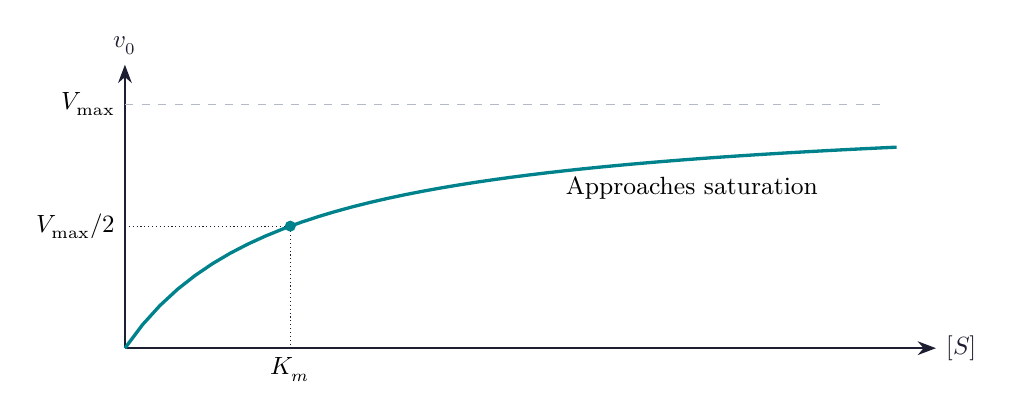
\begin{tikzpicture}[every node/.style={font=\small}]
\draw[arrow] (0,0)--(10.3,0) node[right] {$[S]$};
\draw[arrow] (0,0)--(0,3.6) node[above] {$v_0$};
\draw[myteal,very thick,domain=0:9.8,samples=45] plot (\x,{3.1*\x/(2.1+\x)});
\draw[mgframe,dashed] (0,3.1)--(9.7,3.1);
\draw[mydark,densely dotted] (0,1.55)--(2.1,1.55)--(2.1,0);
\fill[myteal] (2.1,1.55) circle (2pt);
\node[left] at (0,3.1) {$V_{\max}$};
\node[left] at (0,1.55) {$V_{\max}/2$};
\node[below] at (2.1,0) {$K_m$};
\node[below] at (7.2,2.30) {Approaches saturation};
\end{tikzpicture}\par
\end{tcolorbox}

\begin{itemize}[leftmargin=*, itemsep=3pt, topsep=4pt]
  \item \textbf{Units.} $K_m$ is concentration, $V_{\max}$ is concentration per time, and $k_{\mathrm{cat}}$ is inverse time.
  \item \textbf{At half saturation.} $[S]=K_m$ gives $v_0=V_{\max}/2$. It is not generally a pure binding affinity.
  \item \textbf{At low substrate.} $v_0\approx(k_{\mathrm{cat}}/K_m)[E]_T[S]$. The ratio compares catalytic efficiency in the low-substrate limit.
  \item \textbf{Why measure parameters?} They help compare biological reactions, predict rate at a given substrate level, and distinguish reduced turnover from altered apparent substrate dependence.
\end{itemize}
\begin{tcolorbox}[examplebox, title={Calculate rate and turnover}]
If $V_{\max}=12\,\mu\mathrm{M\,s^{-1}}$ and $K_m=3\,\mathrm{mM}$, then at $[S]=6\,\mathrm{mM}$ the rate is $12(6)/(3+6)=8\,\mu\mathrm{M\,s^{-1}}$. If $[E]_T=0.20\,\mu\mathrm M$, the turnover number is $12/0.20=60\,\mathrm{s^{-1}}$.
\end{tcolorbox}

\subsection{Interpret enzyme measurements and common rate changes}
\begin{tcolorbox}[examplebox, title={Convert a time trace into an initial rate}]
In an illustrative measurement, product rises from $2$ to $8\,\mu\mathrm M$ in the first $3\,\mathrm s$ with an approximately straight trace. The initial rate estimate is $(8-2)/3=2\,\mu\mathrm{M\,s^{-1}}$. If the curve later bends, averaging over the entire trace may give a different value. Report the early slope and the units used for concentration and time.
\end{tcolorbox}

\par\vspace{6pt}
\noindent\begin{tabularx}{\linewidth}{|B{3.3cm}|Y|Y|}
\hline
\textbf{Change} & \textbf{Expected result in the simple model} & \textbf{Reason} \\ \hline
More enzyme at the same substrate level & $V_{\max}$ increases with $[E]_T$ while $K_m$ is unchanged. & There are more catalytic sites. Each site follows the same model. \\ \hline
More substrate at fixed enzyme level & The initial rate approaches $V_{\max}$. & Most active sites are occupied at high substrate. \\ \hline
Ideal competitive inhibition & Apparent $K_m$ rises while $V_{\max}$ stays the same. & Substrate and inhibitor compete for free enzyme. \\ \hline
Pure noncompetitive inhibition & Apparent $V_{\max}$ falls while $K_m$ stays the same. & This ideal special case reduces usable catalytic capacity. Other mixed inhibition patterns can affect both quantities. \\ \hline
\end{tabularx}\par

\begin{tcolorbox}[masonbox, title={Connect structure to the kinetics}]
A low value of $K_m$ means half-maximal rate is reached at a lower substrate concentration under the stated model. It is not automatically a binding constant. Compare $k_{\mathrm{cat}}$ when the question is about turnover per active site, and $k_{\mathrm{cat}}/K_m$ for the low-substrate limit.
\end{tcolorbox}

\subsection{RNA catalysis}
\begin{tcolorbox}[defbox, title={Ribozyme}]
A ribozyme is a folded RNA that catalyses a reaction. Its shape positions substrates and reactive groups. Some catalytic RNAs depend on associated ions or proteins.
\end{tcolorbox}

RNase P has a catalytic RNA component involved in processing precursor tRNAs in many organisms. The ribosomal RNA at the large-subunit catalytic centre participates in peptide-bond formation. These examples connect information-processing molecules with chemical catalysis.

\subsection{Explain how RNA can act as a catalyst}
\begin{itemize}[leftmargin=*, itemsep=2pt]
  \item \textbf{Fold.} Base pairing and tertiary contacts bring reactive groups into a definite three-dimensional arrangement.
  \item \textbf{Position.} Folded RNA can bring reactants together and orient them. Metal ions can help stabilise charge in some ribozymes.
  \item \textbf{Illustrate.} RNase P processes precursor tRNA, a self-splicing intron can promote its own removal, and the ribosomal catalytic centre participates in peptide-bond formation. These examples show distinct catalytic roles for RNA.
\end{itemize}

\textbf{Reading.} \href{https://iubmb.qmul.ac.uk/kinetics/}{IUBMB kinetic terminology} and \href{https://www.nobelprize.org/uploads/2018/06/cech-lecture.pdf}{Cech's lecture on RNA catalysis}.

\newpage
\begin{center}
  {\large\bfseries\color{myred} Quick Revision --- Module 5}\\[3pt]
  {\small\color{mydark} Enzymes $|$ BS-B401}
\end{center}
\noindent{\color{myred}\rule{\linewidth}{1.2pt}}\par\vspace{4pt}

\begin{tcolorbox}[formulabox, title={Key Concepts at a Glance}]
\renewcommand{\arraystretch}{1.35}
\noindent\begin{tabularx}{\linewidth}{B{4.5cm}Y}
Michaelis--Menten & $v_0=V_{\max}[S]/(K_m+[S])$. \\[3pt]
Half-maximal velocity & $[S]=K_m$ gives $v_0=V_{\max}/2$. \\[3pt]
Turnover & $k_{\mathrm{cat}}=V_{\max}/[E]_T$. \\[3pt]
\end{tabularx}\par
\end{tcolorbox}

\begin{tcolorbox}[defbox, title={One-Line Definitions}]
\begin{itemize}[leftmargin=*, itemsep=3pt, topsep=4pt]
  \item \textbf{Active site.} Region that binds substrate and supports catalysis.
  \item \textbf{Initial rate.} Early slope of product formation or substrate disappearance.
  \item \textbf{Ribozyme.} Catalytic RNA.
\end{itemize}
\end{tcolorbox}

\begin{tcolorbox}[exambox, title={Frequently Asked / Viva Questions}]
\begin{enumerate}[topsep=0pt, label=\textbf{Q\arabic*.}, itemsep=5pt, leftmargin=*]
  \item \Q{What barrier does an enzyme lower?}
    The activation free-energy barrier.
  \item \Q{Does an enzyme change equilibrium?}
    It changes the approach rate. Equilibrium is set by energetics.
  \item \Q{What is induced fit?}
    Binding changes or selects conformations suited to catalysis.
  \item \Q{What reaction does lactase catalyse?}
    Hydrolysis of lactose to glucose and galactose.
  \item \Q{What supports catalysis in carbonic anhydrase?}
    A zinc ion helps activate water.
  \item \Q{What variable is monitored to determine a rate?}
    A signal that tracks product formation or substrate loss.
  \item \Q{Why use initial rate?}
    Little product has built up and substrate depletion is small.
  \item \Q{What are the units of turnover number?}
    Inverse time.
  \item \Q{Which new class involves membrane movement?}
    Translocases, EC 7.
  \item \Q{Give one example of catalytic RNA.}
    The RNA component of RNase P.
\end{enumerate}
\end{tcolorbox}

\begin{tcolorbox}[tikzbox, title={Summary Comparison}]
\par\vspace{5pt}
\begingroup
\setlength{\extrarowheight}{1pt}
\noindent\begin{tabularx}{\linewidth}{|B{3.45cm}|Y|Y|}
\hline
\textbf{Feature} & \textbf{Protein enzyme} & \textbf{Ribozyme} \\ \hline
Catalytic component & Folded polypeptide. & Folded RNA. \\ \hline
Examples & Lactase or carbonic anhydrase. & RNase P RNA or catalytic ribosomal RNA. \\ \hline
\end{tabularx}\par
\endgroup
\end{tcolorbox}


% -- Module 6 -----------------------------------------------------------------
\modulestart{6}{Information Transfer}

\section{Information Transfer}
\subsection{Evidence that DNA carries hereditary information}
\begin{tcolorbox}[defbox, title={Hereditary material}]
A hereditary molecule stores information, can be copied, can vary, and can be transmitted. DNA is the hereditary material of cellular organisms. Some viruses use RNA as their genome.
\end{tcolorbox}

\par\vspace{5pt}
\begingroup
\setlength{\extrarowheight}{1pt}
\noindent\begin{tabularx}{\linewidth}{|B{3.5cm}|Y|Y|}
\hline
\textbf{Study} & \textbf{Observation in outline} & \textbf{Interpretation} \\ \hline
Avery, MacLeod and McCarty & A DNA-containing fraction carried a heritable change. Degrading DNA removed that effect. & DNA could transmit a characteristic to descendant cells. \\ \hline
Hershey and Chase & The label associated with genetic material entering the host was chiefly linked to DNA rather than to the viral coat. & DNA carried the genetic instructions in the system studied. \\ \hline
\end{tabularx}\par
\endgroup
\subsection{DNA structure from strand to nucleosome}
\begin{enumerate}[leftmargin=*, itemsep=3pt, topsep=4pt]
  \item \textbf{One strand.} Deoxyribonucleotides are connected by $3'$--$5'$ phosphodiester bonds. The sugar-phosphate backbone is directional and the sequence of bases carries information.
  \item \textbf{Double helix.} Two complementary strands run antiparallel. A pairs with T and G with C through hydrogen bonding. Base stacking also stabilises the helix.
  \item \textbf{Nucleosome.} In eukaryotic chromatin, roughly 147 base pairs of DNA wrap around a histone octamer. Linker DNA lies between nucleosome core particles.
  \item \textbf{Chromatin.} Nucleosomes and associated proteins organise DNA further. Packaging influences accessibility for transcription and replication.
\end{enumerate}
\begin{tcolorbox}[tikzbox, title={Levels of eukaryotic DNA packaging}]
\centering
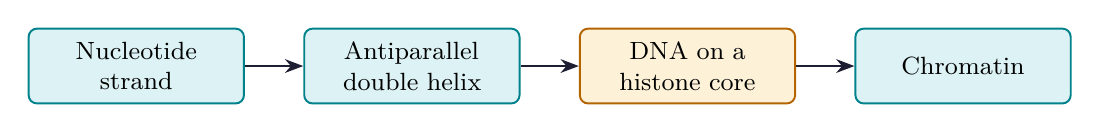
\begin{tikzpicture}[every node/.style={font=\small}]
\node[block,text width=2.5cm] (a) at (0,0) {Nucleotide\\strand};
\node[block,text width=2.5cm] (b) at (3.5,0) {Antiparallel\\double helix};
\node[amberblock,text width=2.5cm] (c) at (7,0) {DNA on a\\histone core};
\node[block,text width=2.5cm] (d) at (10.5,0) {Chromatin};
\draw[arrow] (a)--(b);
\draw[arrow] (b)--(c);
\draw[arrow] (c)--(d);
\end{tikzpicture}\par
\end{tcolorbox}

\section{Expression and the Genetic Code}
\subsection{Replication, transcription and translation}
\par\vspace{5pt}
\begingroup
\setlength{\extrarowheight}{1pt}
\noindent\begin{tabularx}{\linewidth}{|B{3.2cm}|Y|Y|}
\hline
\textbf{Process} & \textbf{Information direction} & \textbf{What to remember} \\ \hline
Replication & DNA to DNA. & Complementarity allows semiconservative copying. Each new duplex has one old strand and one new strand. \\ \hline
Transcription & DNA to RNA. & RNA polymerase reads a template strand and makes complementary RNA. The coding strand matches the transcript over the copied region apart from T versus U. \\ \hline
Translation & mRNA to polypeptide. & The ribosome reads codons. Transfer RNAs match the code and bring amino acids. \\ \hline
\end{tabularx}\par
\endgroup
\begin{tcolorbox}[masonbox, title={Follow direction carefully}]
RNA is synthesised $5'$ to $3'$. A template read in the opposite direction is complementary to the new RNA. Translation reads mRNA from $5'$ to $3'$ and extends a polypeptide from its N terminus to its C terminus.
\end{tcolorbox}

\subsection{What a codon specifies}
\begin{tcolorbox}[defbox, title={Genetic code}]
The genetic code maps each three-base mRNA codon to an amino acid or to a termination signal. A reading frame determines which groups of three are interpreted as codons.
\end{tcolorbox}

\begin{itemize}[leftmargin=*, itemsep=3pt, topsep=4pt]
  \item \textbf{Count.} Four possible RNA bases give $4^3=64$ codons. In the standard code, 61 specify amino acids and UAA, UAG and UGA signal termination.
  \item \textbf{Start.} AUG is the usual start signal in the correct initiation context. In an internal position it typically specifies methionine.
  \item \textbf{Degeneracy.} Several codons can specify the same amino acid. For example, GGU and GGC both specify glycine in the standard code.
  \item \textbf{Near universality.} The standard code is shared widely. Some mitochondria and organisms reassign particular codons, so the code is nearly universal.
  \item \textbf{Reading frame.} During ordinary translation, codons are read consecutively in the chosen frame. A one-base insertion or deletion can change downstream codons.
\end{itemize}
\begin{tcolorbox}[examplebox, title={Read a short illustrative message}]
For the classroom example $5'$--AUG GGU GAA UAA--$3'$, read AUG as the start and methionine, GGU as glycine and GAA as glutamate. UAA ends translation. The peptide is Met--Gly--Glu. The stop signal contributes no amino acid.
\end{tcolorbox}

\subsection{Gene as a functional and a recombination unit}
\begin{itemize}[leftmargin=*, itemsep=3pt, topsep=4pt]
  \item \textbf{Cistron.} In the classical functional definition, mutations that fail to complement in trans are usually assigned to the same functional unit. Mutations in different units may complement if each copy supplies the other's missing function.
  \item \textbf{Cis versus trans.} If two recessive mutations lie on one chromosome in cis, the opposite copy can carry both normal functions. In trans, the mutations lie on opposing copies. Restoration depends on whether functional copies of all required units are present.
  \item \textbf{Recon.} The classical recombination unit is the smallest genetic interval distinguishable by recombination in a given analysis. Recombination can separate sites inside one cistron, so a functional unit may contain many distinguishable sites.
  \item \textbf{Modern interpretation.} A gene is a DNA region contributing to a functional RNA or polypeptide. Regulatory and processing signals help specify when and how that product is made.
\end{itemize}

\subsection{Explain information flow in three stages}
\par\vspace{6pt}
\noindent\begin{tabularx}{\linewidth}{|B{3.1cm}|Y|Y|}
\hline
\textbf{Process} & \textbf{Start and extend} & \textbf{Finish or check} \\ \hline
Replication & Pair each parental strand with a new complementary strand. Both new strands extend in the same chemical direction, although the parental templates are antiparallel. & Each completed duplex retains one old strand. \\ \hline
Transcription & A promoter helps specify where transcription begins. RNA polymerase reads the selected DNA template and grows RNA in the $5'$ to $3'$ direction. & When transcription terminates, the RNA transcript is released. In eukaryotes a precursor transcript may be processed before use. \\ \hline
Translation & Initiation selects a start and fixes the reading frame. During elongation, transfer RNAs bring amino acids and the ribosome joins them. & A stop codon is read by a release factor in ordinary termination, releasing the polypeptide. \\ \hline
\end{tabularx}\par

\begin{tcolorbox}[examplebox, title={Use base pairing to check DNA composition}]
In an ordinary double-stranded DNA sample, suppose adenine makes up 28\% of the bases. Thymine also accounts for 28\%, leaving 44\% for guanine and cytosine together, or 22\% each. The calculation uses pairing across both strands. One individual strand need not have equal amounts of A and T.
\end{tcolorbox}

\subsection{Connect DNA packaging to gene accessibility}
\begin{itemize}[leftmargin=*, itemsep=2pt]
  \item \textbf{Core histones.} The nucleosome octamer contains two copies each of H2A, H2B, H3 and H4. DNA wraps around it, reducing the space needed to package a long molecule.
  \item \textbf{Linker DNA.} Short DNA segments connect successive core particles. Linker histone H1 can associate with this region and help organise chromatin.
  \item \textbf{Accessibility.} Packaging changes how readily proteins contact DNA. This can affect gene expression without changing the sequence of DNA bases.
\end{itemize}

\textbf{Structural reference.} \href{https://www.nature.com/articles/38444}{Luger et al., nucleosome core structure}.
\begin{tcolorbox}[masonbox, title={Keep the three meanings distinct}]
A codon is a triplet read during translation. A cistron is the classical functional unit inferred through complementation. A recon describes resolution in a recombination analysis. Several distinguishable recombination sites may lie within a single functional unit.
\end{tcolorbox}

\newpage
\begin{center}
  {\large\bfseries\color{myred} Quick Revision --- Module 6}\\[3pt]
  {\small\color{mydark} Information Transfer $|$ BS-B401}
\end{center}
\noindent{\color{myred}\rule{\linewidth}{1.2pt}}\par\vspace{4pt}

\begin{tcolorbox}[formulabox, title={Key Concepts at a Glance}]
\renewcommand{\arraystretch}{1.35}
\noindent\begin{tabularx}{\linewidth}{B{4.5cm}Y}
DNA pairing & A--T and G--C, with antiparallel backbones. \\[3pt]
Direction & DNA/RNA synthesis extends the $3'$ end. \\[3pt]
Code & 64 triplets, including three stop codons in the standard code. \\[3pt]
\end{tabularx}\par
\end{tcolorbox}

\begin{tcolorbox}[defbox, title={One-Line Definitions}]
\begin{itemize}[leftmargin=*, itemsep=3pt, topsep=4pt]
  \item \textbf{Codon.} Three-base mRNA unit interpreted during translation.
  \item \textbf{Nucleosome.} DNA wrapped around a histone core.
  \item \textbf{Cistron.} A classical functional unit defined by complementation.
\end{itemize}
\end{tcolorbox}

\begin{tcolorbox}[exambox, title={Frequently Asked / Viva Questions}]
\begin{enumerate}[topsep=0pt, label=\textbf{Q\arabic*.}, itemsep=5pt, leftmargin=*]
  \item \Q{What did the DNA-fraction study establish?}
    DNA could carry a heritable difference in the studied system.
  \item \Q{What does antiparallel mean?}
    The two strands have opposite backbone directions.
  \item \Q{How is DNA first compacted around histones?}
    It wraps around a histone octamer in the nucleosome core.
  \item \Q{Which process makes RNA from a DNA template?}
    Transcription.
  \item \Q{What does tRNA do?}
    It couples codon recognition to delivery of an amino acid.
  \item \Q{Which direction is mRNA read?}
    From $5'$ to $3'$.
  \item \Q{What does degeneracy mean?}
    More than one codon can specify the same amino acid.
  \item \Q{Is the code identical in every biological context?}
    Some organelles and organisms use codon reassignments.
  \item \Q{What is a frameshift?}
    A change in the grouping of downstream codons.
  \item \Q{Can a functional gene contain more than one recombination site?}
    Yes. Recombination can distinguish sites within a cistron.
\end{enumerate}
\end{tcolorbox}

\begin{tcolorbox}[tikzbox, title={Summary Comparison}]
\par\vspace{5pt}
\begingroup
\setlength{\extrarowheight}{1pt}
\noindent\begin{tabularx}{\linewidth}{|B{3.45cm}|Y|Y|}
\hline
\textbf{Process} & \textbf{Template or input} & \textbf{Main output} \\ \hline
Replication & DNA & DNA. \\ \hline
Transcription & DNA & RNA. \\ \hline
Translation & mRNA and amino acids & Polypeptide. \\ \hline
\end{tabularx}\par
\endgroup
\end{tcolorbox}


% -- Module 7 -----------------------------------------------------------------
\modulestart{7}{Macromolecular Analysis}

\section{Macromolecular Analysis}
\subsection{What a reductionistic analysis asks}
\begin{tcolorbox}[defbox, title={Reductionistic analysis}]
Study a complex biological process by isolating its components and asking what each contributes. Combine measurements of the components to explain the behaviour of the whole system. Check whether the isolated behaviour still applies in the cellular context.
\end{tcolorbox}

\begin{enumerate}[leftmargin=*, itemsep=3pt, topsep=4pt]
  \item \textbf{Define the biological task.} For example, ask how a protein recognises oxygen, an ion or a hormone.
  \item \textbf{Identify the component.} Distinguish the polypeptide sequence from its partners, attached small molecules and surrounding membrane or solvent.
  \item \textbf{Compare structures and functions.} Check whether a structural observation predicts a measurable function.
  \item \textbf{Test the explanation.} Compare conditions or naturally occurring variants, then distinguish direct effects on the active site from effects on folding, stability or expression.
\end{enumerate}
\subsection{The four levels of protein structure}
\par\vspace{5pt}
\begingroup
\setlength{\extrarowheight}{1pt}
\noindent\begin{tabularx}{\linewidth}{|B{3.1cm}|Y|Y|}
\hline
\textbf{Level} & \textbf{What is organised} & \textbf{Forces or examples} \\ \hline
Primary & Amino-acid sequence of a polypeptide, written N to C. & Peptide bonds form the backbone. Side-chain order constrains folding. \\ \hline
Secondary & Local backbone patterns such as alpha helices and beta sheets. & Hydrogen bonds between backbone carbonyl and amide groups. Turns connect elements. \\ \hline
Tertiary & Overall three-dimensional arrangement of one polypeptide chain. & Hydrophobic effects, ionic interactions, hydrogen bonds, van der Waals contacts and some disulfide bonds. \\ \hline
Quaternary & Association of several polypeptide chains into one functional assembly. & Interfaces between subunits. Adult haemoglobin has two alpha and two beta chains. \\ \hline
\end{tabularx}\par
\endgroup
\begin{tcolorbox}[tikzbox, title={Read protein structure by scale}]
\centering
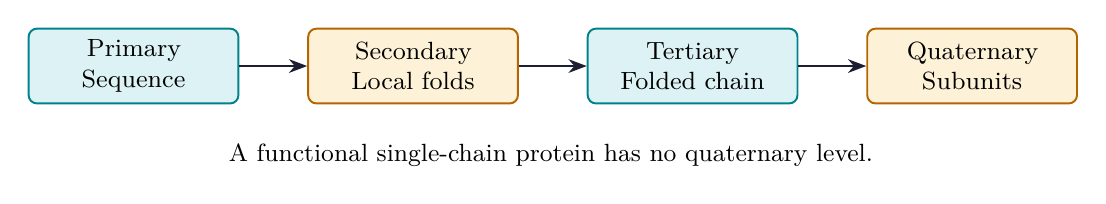
\begin{tikzpicture}[every node/.style={font=\small}]
\node[block,text width=2.43cm] (a) at (0,0) {Primary\\Sequence};
\node[amberblock,text width=2.43cm] (b) at (3.55,0) {Secondary\\Local folds};
\node[block,text width=2.43cm] (c) at (7.1,0) {Tertiary\\Folded chain};
\node[amberblock,text width=2.43cm] (d) at (10.65,0) {Quaternary\\Subunits};
\draw[arrow] (a)--(b);
\draw[arrow] (b)--(c);
\draw[arrow] (c)--(d);
\node at (5.3,-1.13) {A functional single-chain protein has no quaternary level.};
\end{tikzpicture}\par
\end{tcolorbox}

\begin{itemize}[leftmargin=*, itemsep=3pt, topsep=4pt]
  \item \textbf{Alpha helix.} The backbone coils with hydrogen bonds between residues separated by four positions along the chain. Side chains project outward.
  \item \textbf{Beta sheet.} Backbone segments align side by side. Hydrogen bonds connect the strands, which may run parallel or antiparallel.
  \item \textbf{Domains.} A domain is a compact structural unit within a chain. A protein can have several domains with different activities, such as binding and catalysis.
  \item \textbf{Denaturation.} Heat or a chemical change may disrupt native folding and subunit interactions. Ordinary denaturation can abolish activity while leaving most peptide bonds intact.
\end{itemize}
\section{Protein Functions and How to Compare Them}
\subsection{Function depends on structure}
\par\vspace{5pt}
\begingroup
\setlength{\extrarowheight}{1pt}
\noindent\begin{tabularx}{\linewidth}{|B{3.1cm}|Y|Y|}
\hline
\textbf{Role} & \textbf{Structure--function link} & \textbf{Example} \\ \hline
Enzyme & A folded active site brings reactive groups into the right positions. & Carbonic anhydrase accelerates carbon dioxide hydration. \\ \hline
Transporter & A binding site or pore selects a substance. Some transporters use alternating access and energy coupling. & A glucose carrier helps glucose cross a membrane. Haemoglobin transports oxygen in blood. \\ \hline
Receptor & A specific ligand changes the receptor's conformation or interactions and triggers signalling. & The insulin receptor detects insulin and initiates intracellular signalling. \\ \hline
Structural & Fibres and networks resist or distribute forces. & Collagen triple helices contribute to connective-tissue strength. \\ \hline
\end{tabularx}\par
\endgroup
\begin{tcolorbox}[examplebox, title={Separate binding from cooperative behaviour}]
Myoglobin is a single-chain oxygen-binding protein. Haemoglobin contains several subunits. Oxygen binding at one haemoglobin subunit can increase the affinity of the others, giving cooperative binding. This comparison connects a quaternary assembly to a function that cannot be explained by counting identical independent sites alone.
\end{tcolorbox}

\subsection{What common measurements reveal}
\par\vspace{5pt}
\begingroup
\setlength{\extrarowheight}{1pt}
\noindent\begin{tabularx}{\linewidth}{|B{3.6cm}|Y|Y|}
\hline
\textbf{Method} & \textbf{What it can show} & \textbf{Limit} \\ \hline
Gel electrophoresis under denaturing conditions & Approximate chain masses or the presence of several polypeptide species. & Native associations and activity may be lost during analysis. \\ \hline
Size-exclusion chromatography & Relative hydrodynamic size of species in solution. & Shape affects the estimate. Size alone may not establish subunit count. \\ \hline
X-ray crystallography, NMR or cryo-EM & Complementary structural information at different scales and in different conditions. & A structural model must be interpreted with sample conditions and resolution in mind. \\ \hline
Binding or activity assay & Whether ligand binding or catalytic function is measurable. & A low signal may reflect poor folding, low protein amount or a direct functional defect. \\ \hline
\end{tabularx}\par
\endgroup
\begin{tcolorbox}[masonbox, title={Exam response pattern}]
For a structure--function answer, name the structural level, identify the relevant feature, explain the physical consequence, and give a specific biological example.
\end{tcolorbox}

\subsection{Distinguish a channel, a carrier, a pump and a receptor}
\par\vspace{6pt}
\noindent\begin{tabularx}{\linewidth}{|B{3.2cm}|Y|Y|}
\hline
\textbf{Protein role} & \textbf{What changes} & \textbf{What to look for} \\ \hline
Channel & An open pore allows selected ions or molecules through. & Movement through an open channel follows the appropriate electrochemical gradient. \\ \hline
Carrier & A binding site faces one side and then the other. & Binding and conformational change can account for selective, saturable transport. \\ \hline
Pump & Transport is coupled to an energy-yielding process. & An ATP-driven pump can maintain a gradient by moving solutes uphill. \\ \hline
Receptor & A ligand selects or changes a receptor state. & Signal transmission is the defining function. Some receptors also include a channel, so the roles can overlap. \\ \hline
\end{tabularx}\par

\begin{tcolorbox}[examplebox, title={Distinguish binding from signalling}]
Suppose a receptor variant binds the same amount of ligand as the usual receptor but gives a smaller downstream response. Normal binding is evidence that ligand recognition still works under the conditions tested. A changed response suggests a problem with coupling, receptor abundance at the relevant surface, or a downstream partner. Measuring binding alone cannot distinguish these explanations.
\end{tcolorbox}

\subsection{Connect a measurement to the affected structural level}
\begin{enumerate}[leftmargin=*, itemsep=2pt]
  \item \textbf{Check the chain.} If a denaturing measurement shows the expected chain mass, major loss of the polypeptide is less likely. That result alone does not establish correct folding.
  \item \textbf{Check the assembly.} A structural or solution measurement can indicate whether the expected subunits associate. Different assemblies can contain the same chain types.
  \item \textbf{Check function.} Read out binding, catalytic activity or transport, and compare the result with the structure. An unchanged sequence can still yield a different response if the environment or assembly differs.
  \item \textbf{Apply this to haemoglobin.} A single chain can bind oxygen with its haem group. The multi-subunit assembly lets binding at one site influence other sites, which explains why the response depends on more than the number of binding sites.
\end{enumerate}

\newpage
\begin{center}
  {\large\bfseries\color{myred} Quick Revision --- Module 7}\\[3pt]
  {\small\color{mydark} Macromolecular Analysis $|$ BS-B401}
\end{center}
\noindent{\color{myred}\rule{\linewidth}{1.2pt}}\par\vspace{4pt}

\begin{tcolorbox}[formulabox, title={Key Concepts at a Glance}]
\renewcommand{\arraystretch}{1.35}
\noindent\begin{tabularx}{\linewidth}{B{4.5cm}Y}
Primary to quaternary & Sequence, local backbone pattern, one chain's fold, then any subunit assembly. \\[3pt]
Hydrogen bonding & Backbone hydrogen bonds stabilise alpha helices and beta sheets. \\[3pt]
Function & Identify the site, interaction or assembly that enables the task. \\[3pt]
\end{tabularx}\par
\end{tcolorbox}

\begin{tcolorbox}[defbox, title={One-Line Definitions}]
\begin{itemize}[leftmargin=*, itemsep=3pt, topsep=4pt]
  \item \textbf{Domain.} Compact structural unit within a protein chain.
  \item \textbf{Denaturation.} Loss of native structure and often activity.
  \item \textbf{Cooperativity.} Binding at one site influences binding at another.
\end{itemize}
\end{tcolorbox}

\begin{tcolorbox}[exambox, title={Frequently Asked / Viva Questions}]
\begin{enumerate}[topsep=0pt, label=\textbf{Q\arabic*.}, itemsep=5pt, leftmargin=*]
  \item \Q{What is primary structure?}
    The amino-acid order in a polypeptide.
  \item \Q{What stabilises regular secondary structures?}
    Hydrogen bonds between backbone groups.
  \item \Q{How do tertiary and quaternary structure differ?}
    Tertiary structure is one chain's fold. Quaternary structure describes multiple subunits.
  \item \Q{Which protein illustrates an alpha-two beta-two assembly?}
    Adult haemoglobin.
  \item \Q{Does denaturation necessarily break peptide bonds?}
    Most peptide bonds may remain intact while folding is lost.
  \item \Q{What structural feature often determines enzyme specificity?}
    The shape and chemistry of the active site.
  \item \Q{How does a receptor act?}
    Ligand recognition changes its state and initiates signalling.
  \item \Q{Give a structural protein example.}
    Collagen.
  \item \Q{Why compare structure with an activity assay?}
    The structure suggests a mechanism. The assay tests whether it functions.
  \item \Q{What does a reductionistic study still need to consider?}
    Interactions and conditions that matter in the intact system.
\end{enumerate}
\end{tcolorbox}

\begin{tcolorbox}[tikzbox, title={Summary Comparison}]
\par\vspace{5pt}
\begingroup
\setlength{\extrarowheight}{1pt}
\noindent\begin{tabularx}{\linewidth}{|B{3.45cm}|Y|Y|}
\hline
\textbf{Level} & \textbf{Subject} & \textbf{Example} \\ \hline
Secondary & Local backbone geometry & Alpha helix. \\ \hline
Tertiary & One chain's three-dimensional fold & Folded myoglobin. \\ \hline
Quaternary & Multiple chains & Haemoglobin assembly. \\ \hline
\end{tabularx}\par
\endgroup
\end{tcolorbox}


% -- Module 8 -----------------------------------------------------------------
\modulestart{8}{Metabolism}

\section{Metabolism}
\subsection{Thermodynamics in an open biological system}
\begin{tcolorbox}[defbox, title={Metabolism}]
Metabolism is the network of chemical reactions that supplies materials and energy. Catabolic reactions break down molecules and often release usable free energy. Anabolic reactions build molecules and generally need energy input. Cells exchange matter and energy with their surroundings.
\end{tcolorbox}

\par\vspace{5pt}
\begingroup
\setlength{\extrarowheight}{1pt}
\noindent\begin{tabularx}{\linewidth}{|B{3.25cm}|Y|Y|}
\hline
\textbf{Description} & \textbf{Criterion} & \textbf{Meaning} \\ \hline
Exothermic / endothermic & $\Delta H<0$ / $\Delta H>0$. & Heat released or absorbed at constant pressure. \\ \hline
Exergonic / endergonic & $\Delta G<0$ / $\Delta G>0$. & Forward direction is thermodynamically favourable or unfavourable under the stated conditions. \\ \hline
Equilibrium & $\Delta G=0$ and $Q=K_{\mathrm{eq}}$. & No net change. Forward and reverse processes balance. \\ \hline
\end{tabularx}\par
\endgroup
\begin{tcolorbox}[formulabox, title={Actual and standard free energy}]
At uniform temperature and pressure,
\[
\begin{aligned}
\Delta G&=\Delta H-T\Delta S,\\
\Delta G&=\Delta G^\circ+RT\ln Q,\\
\Delta G^\circ&=-RT\ln K_{\mathrm{eq}} .
\end{aligned}
\]
$Q$ is the current activity ratio, whereas $K_{\mathrm{eq}}$ is its equilibrium value. Use kelvin for $T$ and consistent energy units. In biochemistry, a prime as in $\Delta G^{\circ\prime}$ denotes a transformed standard state, often at specified pH, with the corresponding transformed quotient and equilibrium constant.
\end{tcolorbox}

\begin{tcolorbox}[examplebox, title={Calculate a standard free energy}]
At $298\,\mathrm K$, let $K_{\mathrm{eq}}=100$. Then
\[
\begin{aligned}
\Delta G^\circ
  &=-(8.314)(298)\ln(100)\,\mathrm{J\,mol^{-1}}\\
  &\approx -11.4\,\mathrm{kJ\,mol^{-1}} .
\end{aligned}
\]
The standard value favours products. Under actual conditions, use $Q$. If $Q>K_{\mathrm{eq}}$, the forward $\Delta G$ is positive. \textbf{Spontaneity.} A negative actual $\Delta G$ favours forward change. The activation barrier affects its speed.
\end{tcolorbox}

\subsection{ATP, coupling and energy charge}
\begin{itemize}[leftmargin=*, itemsep=3pt, topsep=4pt]
  \item \textbf{Energy currency.} ATP hydrolysis to ADP and inorganic phosphate can drive work or synthesis when reactions are coupled.
  \item \textbf{Add the free-energy changes.} A coupled process is favourable when its combined $\Delta G$ is negative. A shared intermediate or energy-transferring enzyme is needed to link the reactions.
  \item \textbf{Explain hydrolysis.} Free energy depends on the total reactant and product states. Bond breaking alone costs energy. Products can be favoured by factors such as solvation and resonance.
\end{itemize}
\begin{tcolorbox}[examplebox, title={Energy charge of an adenylate pool}]
Energy charge measures adenylates on a scale from 0 (all AMP) to 1 (all ATP):
\[
\begin{aligned}
\mathrm{EC}
 &=\frac{[\mathrm{ATP}]+\frac12[\mathrm{ADP}]}{[\mathrm{ATP}]+[\mathrm{ADP}]+[\mathrm{AMP}]}\\
 &=\frac{3+\frac12(1)}{3+1+1}=0.70
\end{aligned}
\]
for ATP, ADP and AMP concentrations of 3, 1 and 1 mM. The ratio has no units. A rise in ATP relative to AMP raises the charge.
\end{tcolorbox}

\section{Glucose Breakdown and Photosynthesis}
\subsection{Aerobic oxidation of glucose}
\begin{tcolorbox}[formulabox, title={Overall carbon and oxygen balance}]
\[
\mathrm{C_6H_{12}O_6+6O_2\to6CO_2+6H_2O}.
\]
The equation describes the net outcome. The stages transfer energy into ATP and reduced electron carriers.
\end{tcolorbox}

\par\vspace{5pt}
\begingroup
\setlength{\extrarowheight}{1pt}
\noindent\begin{tabularx}{\linewidth}{|B{3.5cm}|Y|Y|}
\hline
\textbf{Stage} & \textbf{Main events per glucose} & \textbf{Where it occurs in a typical eukaryotic cell} \\ \hline
Glycolysis & One glucose yields two pyruvate, net two ATP and two NADH. The energy-investment phase spends ATP before the payoff phase makes more. & Cytosol. \\ \hline
Pyruvate oxidation & Two pyruvate produce two acetyl-CoA, two carbon dioxide and two NADH. & Mitochondrial matrix. \\ \hline
Krebs cycle & Two acetyl groups yield four carbon dioxide, six NADH, two FADH2 and two ATP/GTP equivalents. Oxaloacetate is regenerated. & Mainly mitochondrial matrix. \\ \hline
Electron transport and ATP synthesis & Electrons from reduced carriers ultimately reduce oxygen to water. The proton gradient drives ATP synthase. & Inner mitochondrial membrane. \\ \hline
\end{tabularx}\par
\endgroup
\begin{tcolorbox}[masonbox, title={Keep the roles separate}]
Glycolysis does not require oxygen directly. Oxygen supports aerobic oxidation as the terminal electron acceptor in the respiratory chain. Most ATP in typical aerobic oxidation comes from oxidative phosphorylation, and the exact overall yield can vary.
\end{tcolorbox}

\subsection{Track carbon and electron carriers without memorising an ATP total}
\begin{tcolorbox}[tikzbox, title={Carbon flow during aerobic glucose oxidation}]
\centering
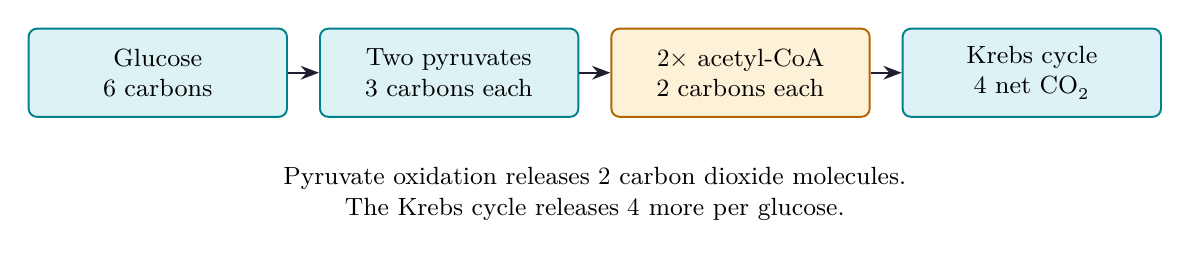
\begin{tikzpicture}[every node/.style={font=\small},
  carbonstep/.style={text width=3cm,minimum height=1.12cm,inner sep=4pt}]
\node[block,carbonstep] (a) at (0,0) {Glucose\\6 carbons};
\node[block,carbonstep] (b) at (3.7,0) {Two pyruvates\\3 carbons each};
\node[amberblock,carbonstep] (c) at (7.4,0) {$2\times$ acetyl-CoA\\2 carbons each};
\node[block,carbonstep] (d) at (11.1,0) {Krebs cycle\\4 net $\mathrm{CO_2}$};
\draw[arrow] (a)--(b);
\draw[arrow] (b)--(c);
\draw[arrow] (c)--(d);
\node[align=center] at (5.55,-1.54) {Pyruvate oxidation releases $2$ carbon dioxide molecules.\\The Krebs cycle releases $4$ more per glucose.};
\end{tikzpicture}\par
\end{tcolorbox}

\begin{itemize}[leftmargin=*, itemsep=2pt]
  \item \textbf{Glycolysis.} Glucose splits into two three-carbon molecules, with no net carbon dioxide release. Substrate-level phosphorylation transfers phosphate directly to ADP.
  \item \textbf{Pyruvate oxidation and the cycle.} Pyruvate oxidation drops one carbon per pyruvate. The cycle releases two carbon dioxide molecules per turn while regenerating oxaloacetate. This is a net balance, since newly entered carbon atoms need not be the ones released in the first turn.
  \item \textbf{Oxidative phosphorylation.} NADH and FADH2 carry reducing equivalents. Electron transfer creates a proton gradient, and flow through ATP synthase couples that gradient to ATP formation. Oxygen is the terminal electron acceptor.
\end{itemize}

\subsection{Photosynthesis builds carbohydrate}
\begin{enumerate}[leftmargin=*, itemsep=3pt, topsep=4pt]
  \item \textbf{Capture light.} In oxygenic photosynthesis, light reactions in thylakoid membranes generate ATP and reducing power in the form of NADPH. Splitting water supplies electrons and releases oxygen.
  \item \textbf{Fix carbon.} The Calvin cycle uses carbon dioxide, ATP and NADPH to make triose phosphate and regenerate its carbon dioxide acceptor. Glucose and other carbohydrates can be assembled from the triose products.
  \item \textbf{Read the net equation.} A simplified net representation is
 \[
 \mathrm{6CO_2+6H_2O \xrightarrow{light} C_6H_{12}O_6+6O_2}.
 \]
 The oxygen released in oxygenic photosynthesis originates from water. The equation summarises the energy-consuming carbon synthesis.
\end{enumerate}
\par\vspace{5pt}
\begingroup
\setlength{\extrarowheight}{1pt}
\noindent\begin{tabularx}{\linewidth}{|B{3.45cm}|Y|Y|}
\hline
\textbf{Pathway} & \textbf{Carbon direction} & \textbf{Energy relationship} \\ \hline
Aerobic respiration & Reduced carbon in glucose is oxidised to carbon dioxide. & Energy-yielding overall, with useful energy transferred to ATP. \\ \hline
Oxygenic photosynthesis & Carbon dioxide is reduced to carbohydrate precursors. & Light energy is captured, then ATP and NADPH help drive carbon fixation. \\ \hline
\end{tabularx}\par
\endgroup

\subsection{Work the energy balance in either direction}
\begin{tcolorbox}[examplebox, title={One uphill reaction coupled to ATP hydrolysis}]
Suppose a biosynthetic step has $\Delta G=+14\,\mathrm{kJ\,mol^{-1}}$ and its coupled ATP hydrolysis has $\Delta G=-30\,\mathrm{kJ\,mol^{-1}}$ under the same stated conditions. Add changes in the same stoichiometric amount:
\[
\Delta G_{\mathrm{net}}=14-30=-16\,\mathrm{kJ\,mol^{-1}}.
\]
This predicts favourable forward change when an actual coupling mechanism links the events.
\end{tcolorbox}

\begin{itemize}[leftmargin=*, itemsep=2pt]
  \item \textbf{Photosynthetic reducing power.} Light reactions produce NADPH, which supplies electrons for reducing fixed carbon, as well as ATP to drive reactions in the Calvin cycle.
  \item \textbf{Carbon-fixation budget.} Fixing three carbon dioxide molecules to yield one net three-carbon triose phosphate uses nine ATP and six NADPH in the standard Calvin cycle count. Two net triose phosphates provide the six carbons needed for a hexose equivalent.
  \item \textbf{Why the cycles differ.} The Krebs cycle oxidises acetyl groups and regenerates oxaloacetate. The Calvin cycle uses chemical energy to fix carbon and regenerates the carbon dioxide acceptor.
\end{itemize}

\textbf{Reading.} \href{https://pubmed.ncbi.nlm.nih.gov/4972613/}{Atkinson's original adenylate energy-charge paper}.

\newpage
\begin{center}
  {\large\bfseries\color{myred} Quick Revision --- Module 8}\\[3pt]
  {\small\color{mydark} Metabolism $|$ BS-B401}
\end{center}
\noindent{\color{myred}\rule{\linewidth}{1.2pt}}\par\vspace{4pt}

\begin{tcolorbox}[formulabox, title={Key Concepts at a Glance}]
\renewcommand{\arraystretch}{1.35}
\noindent\begin{tabularx}{\linewidth}{B{4.5cm}Y}
Gibbs energy & $\Delta G=\Delta G^\circ+RT\ln Q$. \\[3pt]
Equilibrium & $\Delta G^\circ=-RT\ln K_{\mathrm{eq}}$ and actual $\Delta G=0$ at equilibrium. \\[3pt]
Energy charge & $([\mathrm{ATP}]+[\mathrm{ADP}]/2)/([\mathrm{ATP}]+[\mathrm{ADP}]+[\mathrm{AMP}])$. \\[3pt]
\end{tabularx}\par
\end{tcolorbox}

\begin{tcolorbox}[defbox, title={One-Line Definitions}]
\begin{itemize}[leftmargin=*, itemsep=3pt, topsep=4pt]
  \item \textbf{Exergonic.} Forward process with negative Gibbs free-energy change.
  \item \textbf{Catabolism.} Breakdown reactions that often supply usable energy.
  \item \textbf{Anabolism.} Biosynthetic reactions that generally require energy input.
\end{itemize}
\end{tcolorbox}

\begin{tcolorbox}[exambox, title={Frequently Asked / Viva Questions}]
\begin{enumerate}[topsep=0pt, label=\textbf{Q\arabic*.}, itemsep=5pt, leftmargin=*]
  \item \Q{Is every exothermic reaction exergonic?}
    The entropy term can change the sign of Gibbs energy.
  \item \Q{What does negative actual delta G predict?}
    The forward direction is thermodynamically favoured under those conditions.
  \item \Q{What is the role of ATP coupling?}
    Connect favourable hydrolysis to work or an energetically uphill reaction.
  \item \Q{Where does glycolysis occur?}
    In the cytosol.
  \item \Q{What is the net glycolytic ATP yield per glucose?}
    Two ATP.
  \item \Q{What enters the Krebs cycle?}
    An acetyl group carried by acetyl-CoA.
  \item \Q{What accepts electrons at the end of aerobic respiration?}
    Molecular oxygen, which is reduced to water.
  \item \Q{What supplies carbon for photosynthetic carbohydrate?}
    Carbon dioxide.
  \item \Q{Where does oxygen from photosynthesis originate?}
    Water.
  \item \Q{What does energy charge near one indicate?}
    The adenylate pool is dominated by ATP.
\end{enumerate}
\end{tcolorbox}

\begin{tcolorbox}[tikzbox, title={Summary Comparison}]
\par\vspace{5pt}
\begingroup
\setlength{\extrarowheight}{1pt}
\noindent\begin{tabularx}{\linewidth}{|B{3.45cm}|Y|Y|}
\hline
\textbf{Stage or measure} & \textbf{Main quantity} & \textbf{Exam distinction} \\ \hline
Glycolysis & Pyruvate and net ATP & Direct oxygen use is unnecessary. \\ \hline
Calvin cycle & Fixed carbon & Consumes ATP and NADPH. \\ \hline
Energy charge & Relative adenylate state & Dimensionless ratio. \\ \hline
\end{tabularx}\par
\endgroup
\end{tcolorbox}


% -- Module 9 -----------------------------------------------------------------
\modulestart{9}{Microbiology}

\section{Microbiology}
\subsection{Single-celled organisms, species and strains}
\begin{tcolorbox}[defbox, title={Microorganism}]
A microorganism is a microscopic biological entity. Here the focus is on cellular microorganisms. A single cell can sense its surroundings, acquire resources, maintain a boundary and reproduce. Many bacteria, archaea, yeasts, unicellular algae and protists carry out their life processes in one cell.
\end{tcolorbox}

\begin{itemize}[leftmargin=*, itemsep=3pt, topsep=4pt]
  \item \textbf{Prokaryotic examples.} Bacteria and archaea are distinct domains. Both lack a membrane-bound nucleus.
  \item \textbf{Eukaryotic examples.} Baker's yeast is a unicellular fungus. Some algae and protists are also unicellular.
  \item \textbf{Species.} A named biological group. For microorganisms that reproduce asexually, shared ancestry, genome relatedness and consistent traits help define groups. Interbreeding alone is not a practical species test here.
  \item \textbf{Strain.} A distinguishable lineage within a species. Strains can have different observable traits while retaining the same species name.
\end{itemize}
\subsection{Identification and classification}
\par\vspace{5pt}
\begingroup
\setlength{\extrarowheight}{1pt}
\noindent\begin{tabularx}{\linewidth}{|B{3.45cm}|Y|Y|}
\hline
\textbf{Evidence} & \textbf{What it shows} & \textbf{Why combine it with other evidence?} \\ \hline
Microscopy and morphology & Cell size, shape, arrangement or visible structures. & Different species may look similar. A single image rarely establishes species. \\ \hline
Staining or cell envelope traits & Differences in cell structures and how they retain a stain. & The grouping is informative but may be shared by many lineages. \\ \hline
Biochemical observations & Characteristic activities or products under defined observations. & Traits can vary with conditions and among strains. \\ \hline
Molecular comparison & Relatedness inferred from marker sequences or broader genomic evidence. & A conserved marker can place an organism in a broad group without resolving closely related strains. \\ \hline
\end{tabularx}\par
\endgroup
\subsection{Microscopy: magnification, contrast and resolution}
\begin{tcolorbox}[defbox, title={Resolution}]
Resolution is the ability to distinguish adjacent points as separate. Magnification is how much larger an image appears, and contrast is how strongly an object differs from its background. Increasing magnification alone does not improve resolution.
\end{tcolorbox}

\par\vspace{5pt}
\begingroup
\setlength{\extrarowheight}{1pt}
\noindent\begin{tabularx}{\linewidth}{|B{3.5cm}|Y|Y|}
\hline
\textbf{Method} & \textbf{Image information} & \textbf{Typical conceptual use} \\ \hline
Bright-field light & Light transmission and visible contrast. & Observe general cell shape or prepared stained material. \\ \hline
Phase contrast & Converts optical phase differences to intensity differences. & See low-contrast transparent cells without requiring a stain for contrast. \\ \hline
Fluorescence & Detects light emitted by fluorescent molecules. & Locate a labelled structure or naturally fluorescent feature. \\ \hline
TEM / SEM & Electrons transmitted through a thin sample (TEM) or signals from a scanned surface (SEM). & TEM reveals internal organisation. SEM primarily shows surface detail. \\ \hline
\end{tabularx}\par
\endgroup
\begin{tcolorbox}[examplebox, title={Separate magnification from resolution}]
A $10\times$ ocular and a $40\times$ objective give total magnification $400\times$. For an idealised light microscope, a common lateral-resolution estimate is $d\approx0.61\lambda/\mathrm{NA}$. At wavelength $550$ nm and numerical aperture $0.65$, $d\approx516$ nm. A smaller $d$ means finer resolvable detail.
\end{tcolorbox}

\section{Ecology, Sterility and Growth}
\subsection{Ecological roles of single-celled organisms}
\begin{itemize}[leftmargin=*, itemsep=3pt, topsep=4pt]
  \item \textbf{Primary production.} Photosynthetic unicellular algae and some bacteria fix carbon and support aquatic food webs.
  \item \textbf{Decomposition.} Microorganisms recycle material from dead organisms and return nutrients to the surroundings.
  \item \textbf{Element cycles.} Different microbial groups transform carbon, nitrogen and sulfur compounds. These transformations affect soil, water and atmospheric chemistry.
  \item \textbf{Associations.} In a mutualism both partners benefit. In commensalism one benefits with little effect on the other. In competition, organisms draw on the same limiting resource.
\end{itemize}
\subsection{Sterilization and types of media}
\begin{tcolorbox}[defbox, title={Sterilization}]
Sterilization aims to eliminate viable microorganisms, including resistant spores. Disinfection reduces or inactivates many microbes on inanimate surfaces. Antisepsis refers to antimicrobial treatment of living tissue. These are different targets of treatment.
\end{tcolorbox}

\par\vspace{5pt}
\begingroup
\setlength{\extrarowheight}{1pt}
\noindent\begin{tabularx}{\linewidth}{|B{3.45cm}|Y|Y|}
\hline
\textbf{Principle} & \textbf{What it does} & \textbf{Distinction} \\ \hline
Moist or dry heat & Inactivates cells by damaging essential structures and macromolecules. & Methods differ in how heat is transferred and how well materials tolerate it. \\ \hline
Filtration & Physically removes retained particles or cells from a stream. & Removal differs from killing. \\ \hline
Radiation or chemical treatment & Causes damage to DNA or essential molecular structures, depending on the method. & Suitability depends on penetration and material compatibility. \\ \hline
\end{tabularx}\par
\endgroup
\begin{tcolorbox}[defbox, title={Growth medium}]
A medium supplies water and chemical components that support a biological measurement or growth. In general it can provide carbon and energy sources, nitrogen, mineral ions and any required growth factors. A solid medium also contains a supporting gel such as agar. Agar is usually a support rather than the main nutrient.
\end{tcolorbox}

\begin{itemize}[leftmargin=*, itemsep=2pt]
  \item \textbf{Defined medium.} Each ingredient and quantity is known, for example specified mineral salts and a carbon compound.
  \item \textbf{Complex medium.} An extract or another ingredient has incompletely known or variable composition.
  \item \textbf{Selective medium.} Favours some groups over others, so only a subset may appear in an observation.
  \item \textbf{Differential medium.} Uses a visible reaction or indicator to distinguish groups.
\end{itemize}

A medium can be liquid or solid, and the physical form is independent of whether its composition is defined or complex. A single formulation can also be both selective and differential.
\subsection{Growth phases and growth kinetics}
\begin{tcolorbox}[tikzbox, title={Conceptual batch growth curve}]
\centering
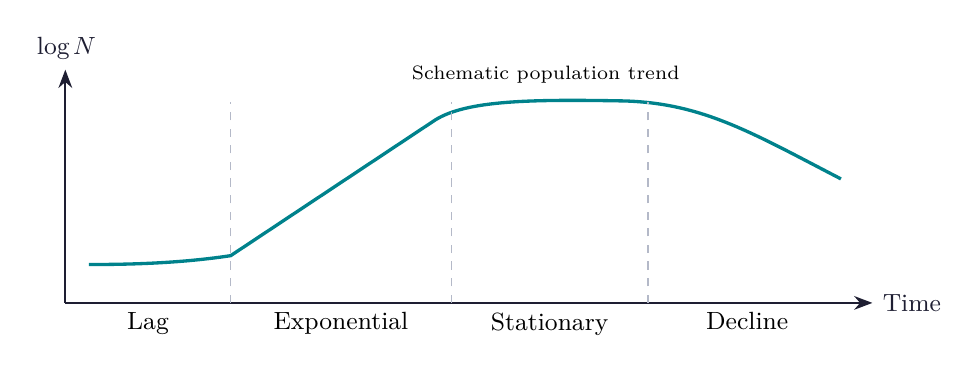
\begin{tikzpicture}[y=0.75cm,every node/.style={font=\small}]
\draw[arrow] (0,0)--(10.25,0) node[right] {Time};
\draw[arrow] (0,0)--(0,3.95) node[above,align=center] {$\log N$};
\draw[myteal,very thick] (0.3,0.65) .. controls (0.9,0.65) and (1.5,0.68) .. (2.1,0.8)
 -- (4.7,3.1) .. controls (5.1,3.43) and (5.9,3.45) .. (7.1,3.42)
 .. controls (8.1,3.38) and (8.72,2.88) .. (9.85,2.1);
\foreach \x in {2.1,4.9,7.4}{\draw[mgframe,dashed] (\x,0)--(\x,3.4);}
\node[below] at (1.05,0) {Lag};
\node[below] at (3.5,0) {Exponential};
\node[below] at (6.15,0) {Stationary};
\node[below] at (8.66,0) {Decline};
\node[font=\scriptsize,align=center] at (6.1,3.86) {Schematic population trend};
\end{tikzpicture}\par
\end{tcolorbox}

\begin{itemize}[leftmargin=*, itemsep=3pt, topsep=4pt]
  \item \textbf{Lag.} Cells adjust to changed conditions. Net population increase may be small.
  \item \textbf{Exponential.} Population increases by a nearly constant proportion per unit time. The log of count is approximately linear.
  \item \textbf{Stationary.} Total viable count levels off when net births and losses nearly balance or division slows.
  \item \textbf{Decline.} Viable count decreases. Total turbidity need not fall at the same rate as viable count.
\end{itemize}
\begin{tcolorbox}[formulabox, title={Exponential growth model}]
With constant specific growth rate $\mu$ and population $N$,
\[
\frac{dN}{dt}=\mu N,\qquad N(t)=N_0e^{\mu t},\qquad
g=\frac{\ln 2}{\mu}.
\]
For discrete doublings, $N=N_0\,2^n$ with $n=t/g$. Here $g$ is the doubling time. This model describes the exponential segment, where the assumptions approximately hold.
\end{tcolorbox}

\begin{tcolorbox}[examplebox, title={Read an illustrative population record}]
A hypothetical count increases from 100 to 800 between two measurements two hours apart. Since $800/100=2^3$, the count doubled three times. The apparent doubling time over that interval is $2/3$ hour, or 40 minutes. The specific rate is $\ln(8)/2\approx1.04\,\mathrm{h^{-1}}$. Apply this interpretation only if the interval is approximately exponential.
\end{tcolorbox}

\subsection{Interpret measurements of a microbial population}
\par\vspace{6pt}
\noindent\begin{tabularx}{\linewidth}{|B{3.4cm}|Y|Y|}
\hline
\textbf{Observation} & \textbf{What it represents} & \textbf{Interpretive limit} \\ \hline
Direct cell count & Number of visible cells in the observed sample. & Live and dead cells can both be counted unless viability is distinguished. \\ \hline
Optical density & Light scattering and attenuation by suspended material. & A proxy for total biomass or particles under comparable conditions. It can remain high after viability falls. \\ \hline
Viable count & An estimate of units capable of forming new growth in the measurement. & Clumps can behave as one unit. Some viable cells may not register in the chosen measurement. \\ \hline
\end{tabularx}\par

\begin{tcolorbox}[examplebox, title={Use an exponential-phase graph rather than one final count}]
On a graph of $\ln N$ against time, the slope in the exponential phase is $\mu$:
\[
\begin{aligned}
\ln N(t)&=\ln N_0+\mu t,\\
\mu&=\frac{\ln N_2-\ln N_1}{t_2-t_1}.
\end{aligned}
\]
This follows directly by taking the logarithm of $N(t)=N_0 e^{\mu t}$. A straight line supports a constant-rate model over that interval. Applying the same slope formula across both lag and stationary phases gives an interval average rather than the exponential growth rate.
\end{tcolorbox}

\subsection{Distinguish ecological role, identification and sterility}
\begin{itemize}[leftmargin=*, itemsep=2pt]
  \item \textbf{Ecological role.} A microscopic producer uses light or chemical energy to make organic matter from inorganic carbon. Decomposers return elements to the surroundings. Changes in one group can alter the resources available to another.
  \item \textbf{Identification.} A visible shape or staining pattern supports a broad grouping. A more specific assignment needs independent evidence. Two related strains may share a marker even if a measured trait differs.
  \item \textbf{Sterility.} A clear-looking sample is not evidence of sterility. Microscopy, turbidity and tests for viability address different questions. A physically removed cell and an inactivated cell may have the same effect on a particular count for different reasons.
\end{itemize}

\begin{tcolorbox}[masonbox, title={Answer a growth-curve question in order}]
Label the axes, explain the four phases, and identify which segment supports an exponential model. Then state whether the plotted data represent total cells, a proxy such as turbidity, or a measure of viable units. That choice determines how you explain the stationary and decline phases.
\end{tcolorbox}

\newpage
\begin{center}
  {\large\bfseries\color{myred} Quick Revision --- Module 9}\\[3pt]
  {\small\color{mydark} Microbiology $|$ BS-B401}
\end{center}
\noindent{\color{myred}\rule{\linewidth}{1.2pt}}\par\vspace{4pt}

\begin{tcolorbox}[formulabox, title={Key Concepts at a Glance}]
\renewcommand{\arraystretch}{1.35}
\noindent\begin{tabularx}{\linewidth}{B{4.5cm}Y}
Magnification & Objective magnification times ocular magnification for a simple compound microscope. \\[3pt]
Resolution & Smaller $d$ means finer detail. A common estimate is $0.61\lambda/\mathrm{NA}$. \\[3pt]
Growth & $N=N_0e^{\mu t}$ when $\mu$ is constant. $g=\ln 2/\mu$. \\[3pt]
\end{tabularx}\par
\end{tcolorbox}

\begin{tcolorbox}[defbox, title={One-Line Definitions}]
\begin{itemize}[leftmargin=*, itemsep=3pt, topsep=4pt]
  \item \textbf{Strain.} A distinguishable lineage within a species.
  \item \textbf{Sterilization.} Elimination of viable microorganisms, including resistant spores.
  \item \textbf{Defined medium.} A medium whose chemical components and amounts are specified.
\end{itemize}
\end{tcolorbox}

\begin{tcolorbox}[exambox, title={Frequently Asked / Viva Questions}]
\begin{enumerate}[topsep=0pt, label=\textbf{Q\arabic*.}, itemsep=5pt, leftmargin=*]
  \item \Q{Name a unicellular fungus used as a model.}
    Baker's yeast.
  \item \Q{Can shape alone usually identify a species?}
    Many groups share shapes, so combine independent evidence.
  \item \Q{What controls the ability to distinguish nearby points?}
    Resolution.
  \item \Q{Which method enhances contrast in transparent cells?}
    Phase contrast is one option.
  \item \Q{Name two ecological roles of microorganisms.}
    Primary production and decomposition.
  \item \Q{How do sterilization and disinfection differ?}
    Sterilization targets all viable forms. Disinfection reduces or inactivates many forms on surfaces.
  \item \Q{What does a differential medium reveal?}
    A visible reaction or other feature that distinguishes groups.
  \item \Q{What is the purpose of a solidifying agent?}
    It provides a solid support.
  \item \Q{Which growth phase gives a straight log-count graph?}
    The exponential phase under the constant-rate model.
  \item \Q{How many doublings turn 100 into 800?}
    Three, because the ratio is eight.
\end{enumerate}
\end{tcolorbox}

\begin{tcolorbox}[tikzbox, title={Summary Comparison}]
\par\vspace{5pt}
\begingroup
\setlength{\extrarowheight}{1pt}
\noindent\begin{tabularx}{\linewidth}{|B{3.45cm}|Y|Y|}
\hline
\textbf{Growth phase} & \textbf{Main observation} & \textbf{Interpretation} \\ \hline
Lag & Small change in count & Adjustment to conditions. \\ \hline
Exponential & Linear log-count trend & Approximately constant relative growth rate. \\ \hline
Stationary / decline & Plateau or fall in viable count & Net growth is near zero or negative. \\ \hline
\end{tabularx}\par
\endgroup
\end{tcolorbox}


\end{document}
